%%%%%%
%%%%%%
%%      ==============================================
%%      Caderno de Músicas Espíritas (livro_musicas.tex)
%%      ==============================================
%%
%%      Version 1.0, 05 de janeiro de 2011
%%      Baseado no arquivo exemplo do pacote songbook de Christopher Rath
%%      Muito obrigado a ele por nos fornecer tão bacana solução para
%%      se escrever músicas cifradas
%%
%%%%%%
%%%%%%
%%
%%      1. Notação de cifras.  Eeste livro de músicas segue
%%         as seguintes convenções
%%
%%              "Menor" é entrado como "m";
%%                      ex.: Cm7 para C menor com 7ª.
%%              "Maior" é entrado como "M" ou nada;
%%                      ex.: CM7 ou C7 para C maior com 7ª.
%%
%%%%%%
%%%%%%

%%%%%%%%%%%%%%%%%%%%%%%%%%%%%%%%%%%%%%%%%%%%%%%%%%%%%%%%%%
%%%%%%%%%%%%%%%%%%%%%%%%%%%%%%%%%%%%%%%%%%%%%%%%%%%%%%%%%%
%%                                                      %%
%%           P R E A M B L E   B E G I N S              %%
%%                                                      %%
%%%%%%%%%%%%%%%%%%%%%%%%%%%%%%%%%%%%%%%%%%%%%%%%%%%%%%%%%%
%%%%%%%%%%%%%%%%%%%%%%%%%%%%%%%%%%%%%%%%%%%%%%%%%%%%%%%%%%

% 12pt = letras maiores
\documentclass[a4,12pt,oneside]{book}
% 11pt = letras menores
%\documentclass[11pt,oneside]{book}

\usepackage{ucs}
\usepackage[utf8x]{inputenc}
\usepackage[T1]{fontenc}
%\usepackage{ae}
\usepackage[brazil]{babel}
\usepackage{latexsym,fancyhdr}
\usepackage{multicol}
\usepackage{graphicx}
\usepackage{tikz}
\usetikzlibrary{calc}


%%% Escolha uma das opcoes abaixo
%%%
\usepackage[chordbk]{songbook}                %% Com letras e cifras - grande.
%\usepackage[wordbk]{songbook}                 %% Somente letras.
%\usepackage[overhead]{songbook}               %% Sem cabeçalho.
%%%opcao depreciada
%\usepackage[compactsong,chordbk]{songbook}    %% Com letras e cifras - compacto.
%%%

%%% Para colocar diagramas de cifras na música - experimental
\usepackage{texchord}
\bigchords\textchords


%%%
% Definições para Data de Revisão e Data de Lançamento.
%
%       \RelDate - A última vez que este livro de músicas foi lançado
%                  Ajuste isso para a data cada vez que uma nova versão/autalização
%                  deste livro de músicas for gerado.
%       \RevDate - A última vez que uma cançao em particular foi revisada de alguma
%                  forma. Este comando será renovado dentro de cada música.
%%%
\newcommand{\RelDate}{\today}
\newcommand{\RevDate}{\today}

%%%
% C.C.L.I. license number definition; for copyright licensing info.
% One of these macros will be manually inserted into the {CpyRt}
% parameter of the {song} environment.
%
%       \CCLInumber - The actual copyright license number.  Don't
%               insert this command in the {CpyRt} parameter, use one
%               of the others.
%       \CCLIed - Indicates a song falls under our CCLI license.
%       \NotCCLIed - Indicates a song doesn't fall under our CCLI
%               license.  Public Domain songs fall into this category.
%       \PGranted - We have received specific permission from the
%               copyright holder to use this song.
%       \PPending - We are in the process of obtaining permission to
%               use this song.
%%%
%% originais
%\newcommand{\CCLInumber}{CCLI Number}
%\newcommand{\CCLIed}{{\CpyRtInfoFont (CCLI \CCLInumber)}}
%\newcommand{\NotCCLIed}{\relax}
%\newcommand{\PGranted}{\relax}
%\newcommand{\PPending}{{\CpyRtInfoFont (Permissão pendente)}}
%
%% meus valores
\newcommand{\CCLInumber}{\relax}
\newcommand{\CCLIed}{\relax}
\newcommand{\NotCCLIed}{\relax}
\newcommand{\PGranted}{Permitido}
\newcommand{\PPending}{{\CpyRtInfoFont (Permissão pendente)}}

%%%
% Informações da página de título (capa).
%%%
\title{Caderno de Músicas Espíritas}
\author{Grupo Violão Amigo}
\date{Última Revisão do Caderno: \RelDate}

%%%
% Redefine fonts from SongBook style that I don't like.
%%%
\font\myTinySF=cmss8 at 8pt
\renewcommand{\CpyRtInfoFont}{\tiny\myTinySF}


%%%
% Redefine a fonte basica para menor
%
\renewcommand{\ChBassFont}{\small\bf\sf}
\renewcommand{\ChFont}{\normalsize\fontfamily{\sfdefault}\fontseries{sbc}\fontshape{n}\selectfont}
%\renewcommand{\ChBkFont}{\ChFont\fontseries{m}\selectfont}

%%%
% Define fontes para uso nos cabeçalhos e rodapés
%%%
\newcommand{\LHeadFont}{\normalsize}            % = cmr12  at 12pt
\newcommand{\CHeadFont}{\normalsize\rm}         % = cmr12  at 12pt
\newcommand{\RHeadFont}{\normalsize}            % = cmr12  at 12pt
\newcommand{\LFootFont}{\scriptsize}            % = cmr8   at  8pt
\newcommand{\CFootFont}{\tiny\myTinySF}         % = cmss8  at  8pt
\newcommand{\RFootFont}{\scriptsize}            % = cmr8   at  8pt

%%%
% Liga e define página com cabeçalho e rodapé
%%%
\pagestyle{fancy}

\ifChordBk
  % It's a words & chords songbook...
  \addtolength{\headwidth}{\marginparsep}
  \addtolength{\headwidth}{\marginparwidth}
  \renewcommand{\headrulewidth}{0.4pt}
  \renewcommand{\footrulewidth}{0.4pt}
  \fancyhead[LE,RO]{\LHeadFont\emph{\leftmark\/}\SBContinueMark}
%  \fancyhead[CE,CO]{\CHeadFont\thepage}
  \fancyhead[CE,CO]{}
%  \fancyhead[RE,LO]{\RHeadFont\RevDate}
  \fancyhead[RE,LO]{Caderno de Música}
\else\ifOverhead
  % It's an overhead...
  \renewcommand{\footrulewidth}{0pt}
  \renewcommand{\headrulewidth}{0pt}
  \fancyhead[LE,RO]{}
  \fancyhead[CE,CO]{}
  \fancyhead[RE,LO]{}
\else\ifWordBk
  % It's a words only songbook...
  \addtolength{\headwidth}{\marginparsep}
  \addtolength{\headwidth}{\marginparwidth}
  \renewcommand{\headrulewidth}{0.4pt}
  \renewcommand{\footrulewidth}{0.4pt}
  \fancyhead[LE,RO]{\LHeadFont Caderno de Músicas Espíritas}
  \fancyhead[CE,CO]{\CHeadFont\thepage}
%  \fancyhead[RE,LO]{\RHeadFont\RevDate}
  \fancyhead[RE,LO]{Caderno de Música}
\fi\fi\fi

\fancyfoot[LE,RO]{\LFootFont Centro Espírita Chico Xavier}
\ifSongEject
  \fancyfoot[CE,CO]{\CFootFont {Ultima revisao:  \RevDate}}
\else
  \fancyfoot[CE,CO]{\CFootFont}
\fi
\fancyfoot[RE,LO]{\RFootFont Grupo Violão Amigo}

%%%
% Turn on/off index-file generation.  Uncomment the \makeindex line to
% turn index generation on;  comment it out to turn index generation
% off.
%%%
\makeTitleIndex         %% Title and First Line Index.
\makeTitleContents      %% Table of Contents.
%\makeKeyIndex           %% Index of song by key.


%Ajusta o título das músicas para que não apareça a numeração
\renewcommand{\STitle}[3][Y]{%
  \setcounter{SBVerseCnt}{0}%
  \setcounter{SBSectionCnt}{0}%
  \ifExcludeSong\relax%
    \else\keyIndex{{\protect\sbChord#3\protect\relax} -- #2}{\theSBSongCnt}\fi%
  \vspace{\SpaceAboveSTitle}%
  \if#1Y\begin{center}\fi
    %{\STitleNumberFont\theSBSongCnt}%
    {\STitleFont\ #2}%
    \ifWordsOnly\relax\else{\STitleKeyFont\ [{\sbChord#3\relax}]}\fi%
  \if#1Y\end{center}\fi
  \STitleMarkboth{#2}{\relax}%
  }

%%Outros ajustes
\renewcommand{\SBPubDom}{Domínio Público}
\renewcommand{\SBWAndMTag}{Letra e música: }
\renewcommand{\SBChorusTag}{Refrão:}

\renewcommand{\marginparwidth}{0pt}

\newcommand{\diminuto}{{$^{\circ}$}}
\newcommand{\primeira}{{$^{\texttt{a}}$}}


%%%%%%%%%%%%%%%%%%%%%%%%%%%%%%%%%%%%%%%%%%%%%%%%%%%%%%%%%%
%%%%%%%%%%%%%%%%%%%%%%%%%%%%%%%%%%%%%%%%%%%%%%%%%%%%%%%%%%
%%                                                      %%
%%       I N I C I O   D O   D O C U M E N T O          %%
%%                                                      %%
%%%%%%%%%%%%%%%%%%%%%%%%%%%%%%%%%%%%%%%%%%%%%%%%%%%%%%%%%%
%%%%%%%%%%%%%%%%%%%%%%%%%%%%%%%%%%%%%%%%%%%%%%%%%%%%%%%%%%

%\usepackage{showframe}

\begin{document}

%%%
% Descomente a linha do "\maketitle" para produzir uma capa padrão.
% Descomente o titlepage para uma capa mais estilosa
% Use uma ou outra alternativa
%%%
%\maketitle

\newpage
\thispagestyle{empty}
\begin{titlepage}
%	\begin{tikzpicture}[remember picture, overlay]
%	  \draw[line width = 4pt] ($(current page.north west) + (2cm,-2cm)$) rectangle ($(current page.south east) + (-3.2cm,2cm)$);
%	\end{tikzpicture}

	\begin{center}
	
%		\vspace{1cm}
	
		\LARGE{\textbf{\textit{Grupo Espírita}}}
		
		\LARGE{\textbf{\textit{Chico Xavier}}}
		
		\vspace{2cm}
	
		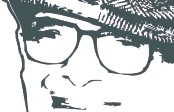
\includegraphics[scale=1.2]{chico.jpg}
		
		\vspace{2cm}
	
		\Large{\textbf{\textit{Escola de Evangelização Infanto-Juvenil}}}
	
		\Large{\textbf{\textit{Grupo Violão Amigo}}}
		
		\vspace{2cm}
		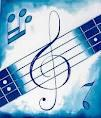
\includegraphics[scale=1.5]{nota.jpg}
		
		\vspace{3cm}
		
		\Large{\textbf{Caderno de Música}}
		\end{center}
\end{titlepage}


%% pagina 2 em branco se twoside
%\newpage
%\thispagestyle{empty}
%\mbox{}

%% TOC
%\newpage
%\thispagestyle{empty}
%{\Large \textbf{Sumário}}
%\begin{description}
%\input{livro_musicas_toc.tex}
%\end{description}



%% pagina 4 em branco se twoside
%\newpage
%\thispagestyle{empty}
%\mbox{}


% reinicia a numeração das páginas para a forma correta
\mainmatter


%% descomente as linhas abaixo para uma forma mais compacta das músicas
%% quando imprimindo somente as letras
\ifWordBk
  \twocolumn
\fi


%%%
% As músicas iniciam aqui.
% Comandos mais usados:
%   \Ch{Cifra}{Sílaba}  - coloca a cifra acima da sílaba na música
%   \Chr{Cifra}{Sílaba} - o mesmo que \Ch, mas emite um traço para completar
%                         um sílaba pequena em relação à cifra
%%%
% Ambientes mais usados
%   \begin{SBVerse}<estrofe>\end{SBVerse} - uma estrofe numerada da música
%   \begin{SBVerse*}<estrofe>\end{SBVerse*} - uma estrofe não numerada da música
%   \begin{SBBracket}{texto}<estrofe>\end{SBBracket} - coloca a estrofe enclausurada com
%                      colchetes ou chaves e o "texto" ao lado, p.ex., BIS, 3X, etc.
%   \begin{SBChorus}<refrao>\end{SBChorus} - refrão da música (coloca "Refrão:" no inicio)
%   \begin{SBChorus*}<refrao>\end{SBChorus*} - refrão da música (não coloca "Refrão:" no inicio)
%   \begin{SBOpGroup}<algo>\end{SBOpGroup} - agrupa algo na música (um open group)
%%%

\setcounter{page}{2}

\begin{song}{A canção que a gente fez}{C}
  {Projeto Carrossel}
  {Movimento Espírita}
  {}
  {\NotCCLIed}

	\renewcommand{\RevDate}{10 de setembro de 2016}
  
	\vspace{-1em}
	
	\SBIntro[N]{{\SBLyricNoteFont C ~ F ~ Am ~ F}\\}
	
	\ifChordBk
		{\vspace{-3em}\flushright{\Amchord \quad \Cchord \quad \Fchord \quad \Gchord}\\}
		\vspace{-1em}
	\fi

	\begin{SBVerse*}
		\Ch{C}{Como} nos velhos tempos de outras tantas

		\Ch{F}{Que} sua vontade sempre permaneça viva

		\Ch{Am}{E} que o amor quebre qualquer  barreira junto com teu \Ch{F}{mar}
	\end{SBVerse*}
	

	\begin{SBVerse*}
		\Ch{C}{Como} nos velhos tempos de outras tantas

		\Ch{F}{Que} seu poder esteja em suas mãos

		\Ch{Am}{E} só dependa de ti pra exerci\Ch{F}{tar}
	\end{SBVerse*}

	\begin{SBVerse*}
		\Ch{C}{Porque} te deténs de sonhar sabe que não pode ter medo de errar

		\Ch{F}{E} a vitória diante de seu olhar está
	\end{SBVerse*}


	\begin{SBVerse*}
		\Ch{C}{Porque} te deténs de amar sabe que não pode viver pra odiar

		\Ch{F}{E} o medo já toma rumo pra outras distâncias ~ AAA...
	\end{SBVerse*}


	\begin{SBVerse*}
		As dores da \Ch{C}{alma} que a gente plantou

		Parecem que \Ch{F}{não} se esquecem de nós

		Mas vamos mu\Ch{Am}{dar}, não vamos nos entregar 
		
		Esse não é o \Ch{F}{fim}
	\end{SBVerse*}
	

	\begin{SBVerse*}
		Os tombos da \Ch{C}{vida} que a gente levou

		Parecem que \Ch{F}{vem} só pra rir de nós

		Mas não vamos de\Ch{Am}{sistir}, não paremos de cantar
		
		A canção que a \Ch{F}{gente} fez
	\end{SBVerse*}


	\begin{SBVerse*}
		\begin{SBBracket*}{2x}
		O momento é \Ch{Am}{hoje}, encoraje o seu ser.

		Ele\Ch{F}{vando} os pensamentos, a uma voz que te cha\Ch{C}{ma}, 
		
		não deixe nada \Ch{G}{te} deter
		\end{SBBracket*}
	\end{SBVerse*}
	
\end{song}


\begin{song}{Alçar voo}{G}
  {Domínio Público}
  {Movimento Espírita}
  {}
  {\NotCCLIed}

	\renewcommand{\RevDate}{20 de abril de 2015}
  
	\SBIntro[N]{\Ch{G}{} \Ch{C}{} \Ch{G}{} \Ch{C}{}}
	
	\ifChordBk
		{\vspace{-3em}\flushright{\Gchord \quad \Cchord \quad \Amchord \quad \Dschord \quad \Bmchord}\\}
		\vspace{-1em}
	\fi

	\begin{SBVerse*}
		Alçar \Ch{G}{voo} é fácil conse\Ch{Am}{guir}

		Molhar as \Ch{C}{mãos} no mar,

		\Ch{D}{Subir} ao céu, re\Ch{G}{gar} o chão.\Ch{D7}{}

		Tuas \Ch{G}{asas} são armas pra vo\Ch{Am}{ar}

		E quem conse\Ch{C}{guir} voar da \Ch{D}{vida} sabe\Ch{G}{rá}
	\end{SBVerse*}


	\begin{SBVerse*}
		\Ch{Am}{Voe} bem mais alto, verás a \Ch{Bm}{Terra}

		A \Ch{Am}{dor}, o sofrimento, verás a \Ch{Bm}{guerra}

		\Ch{C}{Só} assim... tu sabe\Ch{Bm}{rás}

		\Ch{C}{Como} podes aju\Ch{Bm}{dar}...

		Com a \Ch{A}{tua} paz \Ch{D7}{} Ir\Ch{G}{mão}... \Ch{D7}{}

	\end{SBVerse*}


		\begin{SBVerse*}
		{\footnotesize \texttt{(Repete tudo)}

		\texttt{Final:}}
		
		\quad\quad Alçar \Ch{G}{voo}...
	\end{SBVerse*}
	
\end{song}


\begin{song}{Amanhecer}{D}
  {Harmonia}
  {Harmonia}
  {}
  {\NotCCLIed}

	\renewcommand{\RevDate}{12 de maio de 2014}
  
	\SBIntro[N]{\Ch{D}{} \Ch{G}{} \Ch{A7}{} \Ch{D}{} \\ \Ch{A7}{}}
	
	\ifChordBk
		{\vspace{-3em}\flushright{\Dchord \quad \Gchord \quad \Aschord}\\}
		\vspace{-1em}
	\fi

%	\begin{SBOpGroup}
%		Dã dã... dã dã rã dã rã...
%	\end{SBOpGroup}
	
	\begin{SBVerse}
		Por \Ch{D}{mais} que a \Ch{G}{noi}te caia
		
		\Ch{A7}{Sem}pre haverá um novo \Ch{D}{ama}nhecer
		
		E \Ch{D}{então} se\Chr{G}{re}mos fe\Ch{A7}{lizes} por ver o sol nas\Ch{D}{cer}
		
		\Ch{D}{Por} ver a \Ch{G}{luz} chegar
		
		I\Ch{A7}{lumi}nando todos \Ch{D}{os} corações
		
		E en\Ch{D}{tão} fa\Ch{G}{remos} fe\Ch{A7}{lizes} também nossos ir\Ch{D}{mãos}
	\end{SBVerse}
	
	\begin{SBVerse}
		Por \Ch{D}{mais} que a \Ch{G}{noi}te caia
		
		\Ch{A7}{Sem}pre haverá um novo \Ch{D}{ama}nhecer
		
		E \Ch{D}{então} se\Chr{G}{re}mos fe\Ch{A7}{lizes} por ver o sol nas\Ch{D}{cer}
		
		\Ch{D}{Por} ver as \Ch{G}{flo}res
		
		\Ch{A7}{Cheias} de orvalho colo\Ch{D}{rindo} a manhã
		
		E \Ch{D}{uma} can\Ch{G}{ção} vo\Ch{A7}{ando} nas asas da emo\Ch{D}{ção}
	\end{SBVerse}
	
	\begin{SBBracket}{2x}
		Por \Ch{D}{mais} que a \Ch{G}{noi}te caia
		
		E a \Ch{A7}{vida} pareça escure\Ch{D}{cer}...
		
		Por \Ch{D}{mais} que a \Ch{G}{noi}te caia
		
		\Ch{A7}{Um} novo dia vai \Ch{D}{nas}cer
	\end{SBBracket}
\end{song}


\begin{song}{A Paz}{A}
  {\SBPubDom}
  {Grupo Ame}
  {}
  {\NotCCLIed}
  
	\renewcommand{\RevDate}{23 de julho de 2014}

	\SBIntro[N]{\Ch{A}{} \Ch{D}{} \Ch{A/C#}{} \Ch{Bm}{}} 

	\ifChordBk
		{\vspace{-2em}\flushright{\Achord \quad \Dchord \quad \ACsuschord \quad \Bmchord}\\}
		\vspace{-1em}
	\fi
		
	\begin{SBVerse}
		\Chr{D}{Vem} comigo, venha \Chr{A/C#}{lo}go traga o teu olh\Ch{Bm}{ar}
		
		P'ra \Chr{D}{es}ta empreitada \Chr{A/C#}{on}de todos podem \Ch{Bm}{tra}balhar
	\end{SBVerse}
	
	\begin{SBBracket}{}
		A \Chr{D}{paz}, \Chr{A}{a} \Ch{Bm}{paz}
		
		A \Ch{D}{paz}, \Chr{A}{a} \Ch{Bm}{paz} ~ \Ch{A}{}
	\end{SBBracket}
	
	\begin{SBVerse}
		\Ch{D}{Com} o meu esforço, \Ch{A/C#}{com} o teu esforço, \Chr{Bm}{va}mos construir
		
		\Ch{D}{Es}te edifício \Ch{A/C#}{que} ninguém há de \Ch{Bm}{des}truir
	\end{SBVerse}
	
	\begin{SBBracket}{}
		A \Ch{D}{paz}, \Chr{A}{a} \Ch{Bm}{paz}
		
		A \Ch{D}{paz}, \Chr{A}{a} \Ch{Bm}{paz} ~ \Ch{A}{}
	\end{SBBracket}
	
	\begin{SBVerse}
		\Ch{D}{Vem} comigo traga \Ch{A/C#}{a} tua alegria \Ch{Bm}{de} viver
		
		\Ch{D}{Tua} esperança \Ch{A/C#}{a} tua certeza \Ch{Bm}{no} vencer
	\end{SBVerse}
	
	\begin{SBBracket}{2x}
		\Ch{A}{} \Ch{B}{Va}mos \Chr{C#}{cons}tru\Ch{D}{ir} a \Ch{A}{paz} \Ch{Bm}{e o} amor
		
		\Ch{A}{} \Ch{B}{Va}mos \Chr{C#}{cons}tru\Ch{D}{ir} \Ch{A}{um} mundo \Ch{Bm}{me}lhor
	\end{SBBracket}

	\begin{SBOpGroup}
		~ \Ch{A}{~} ~ \Ch{B}{~} ~ \Ch{C#}{ } ~ \\
	\end{SBOpGroup}
\end{song}


\begin{song}{Bem Aqui Onde Estou}{A}
  {\SBPubDom}
  {Elias Brasilino}
  {}
  {\NotCCLIed}
  
	\renewcommand{\RevDate}{25 de setembro de 2014}
 
	\SBIntro[N]{\Ch{D}{} \Ch{A}{} \Ch{Bm}{} \Ch{F#m}{} \Ch{G}{} \Ch{Gm}{} \Ch{A}{}}
	
	\ifChordBk
		{\vspace{-2em}\flushright{\Dchord \quad \Achord \quad \Bmchord 
		    \quad \Fsusmchord \quad \Gchord
		    
		    ~\\
		    
		    \Gmchord}\\}
		\vspace{-3cm}
	\fi

	\begin{SBVerse*}
		\Ch{D}{Sentimentos} \Ch{A}{de} gratidão

		\Ch{Bm}{Por} me sentir de \Ch{F#m}{bem} com a vida

		\Ch{G}{Doce} ambiente de\Ch{Gm}{}emoção

		\Ch{A}{No} fundo de meu coração
	\end{SBVerse*}
	
	\begin{SBVerse*}
		\Ch{D}{Me} fazem olhar pro \Ch{A}{céu}

		\Ch{Bm}{Numa} noite estre\Ch{F#m}{lada}

		\Ch{G}{Ouvindo} as vozes da \Ch{Gm}{noite}

		\Ch{A}{Que} me falam de madrugada
	\end{SBVerse*}
	
	\begin{SBVerse*}
		\Ch{D}{Sinfonia} de \Ch{A}{luzes}

		\Ch{Bm}{Músicas} celes\Ch{F#m}{tiais}

		\Ch{G}{Chuva} incessante de \Ch{Gm}{} amor

		\Ch{A}{Bem} aqui onde estou
		
		~\\
		
	 	{\small
			\texttt{(Repete tudo)}

			\texttt{(Finaliza:} \textbf{D} \texttt{)}
		}
		
	\end{SBVerse*}
\end{song}


\begin{song}{Boa Nova}{D}
  {\SBPubDom}
  {Vital Arguelho Filho}
  {}
  {\NotCCLIed}
  
	\renewcommand{\RevDate}{24 de julho de 2014}
  
	\SBIntro[N]{\Ch{D}{} \Ch{Bm}{} \Ch{G}{} \Ch{A}{} \Ch{[2x]}{}}

	\ifChordBk
		{\vspace{-2em}\flushright{\Dchord \quad \Bmchord \quad \Gchord \quad \Achord \quad \Fsusmchord}\\}
		\vspace{-2em}
	\fi
	
	\begin{SBVerse*}
		(Nara Nana Nana...)
		
		\Ch{D}{Ah...} uma flor se a\Ch{Bm}{bre}
		
	    Ela \Ch{G}{traz} novos aromas pra sentir \Ch{A}{}
	    
	    \Ch{D}{Ah}, uma criança nas\Ch{Bm}{ce,}
	    
	    Ela \Ch{G}{traz} a esperança de um porvir \Ch{A}{}

		Mas a\Ch{Bm}{inda} existe o medo

		A\Ch{F#m}{inda} existe a dor
		
		Ainda e\Ch{G}{xis}te a ignomínia huma\Ch{A}{na}
		
		A Re\Ch{Bm}{vela}ção nos ensina \Ch{F#m}{todos} os porquês
		
		E nos \Ch{G}{mos}tra o caminho a percor\Ch{A}{rer}
    \end{SBVerse*}
    
    \begin{SBChorus}
		Evangeli\Ch{G}{zar}
		
		E um \Ch{A}{mun}do novo cri\Ch{F#m}{ar,} ~ \Ch{Bm}{}
		
		Evangeli\Ch{G}{zar}
		
		Novos \Ch{A}{ru}mos ao planeta \Ch{F#m}{vamos} dar \Ch{Bm}{}
		
		Evangeli\Ch{G}{zar}
		
		É se \Ch{A}{ter} novos aromas \Ch{F#m}{pra} sentir \Ch{Bm}{}

		Evangeli\Ch{G}{zar}
		
		É se \Ch{A}{ter} a esperança \Ch{G}{de\SBen um} \Ch{A}{por}\Ch{D}{vir}
    \end{SBChorus}
	
	\begin{SBOpGroup}
		{\small\texttt{Final:}}{\Ch{D}{Ah...} Uma flor se a\Ch{Bm}{bre...}}
	\end{SBOpGroup}
\end{song}


\begin{song}{Boa Nova}{G}
  {Grupo Sal e Luz}
  {Elias Brasilino}
  {CONJOVEM 2015}
  {\NotCCLIed}
  
	\renewcommand{\RevDate}{15 de abril de 2015}
  
	\SBIntro[N]{\Ch{G}{} \Ch{Bm}{} \Ch{C}{} \Ch{D}{} \Ch{C}{} \Ch{D}{} \Ch{C}{} \Ch{G}{}}
	
	\ifChordBk
		{\vspace{-1em}\flushright{\Gchord \quad \Bmchord \quad \Bmschord \quad \Cchord \quad \Dchord \quad \Emchord
		\quad \Amchord\\}}
	\fi
	
    \begin{SBChorus}
		\ifChordBk
			\vspace{-1cm}
		\fi
		
		\Ch{G}{Eu} Venho \Ch{Bm7}{te chamar}
		
		Pra \Ch{C}{divulgar} \Ch{D}{Bo}\Ch{C}{a} \Ch{D}{No}\Ch{C}{va}
		
		\Ch{G}{Eu} Venho \Ch{Bm7}{te chamar}
				
		Pra \Ch{C}{vivenciar} \Ch{D}{Boa} \Ch{C}{No}\Ch{D}{va} \Ch{C}{}
    \end{SBChorus}

	\ifChordBk
	\begin{flushright}
		\begin{minipage}{0.50\columnwidth}
	\fi
			\begin{SBVerse}
				\ifChordBk
					\vspace{-2.5cm}
				\fi

				\Ch{Em}{Tende} bom \Ch{Bm7}{ânimo}
				
				{\normalsize E \Ch{C}{creia} na Justiça \Ch{Bm7}{}Divina}
				
				\Ch{C}{Exercitando} o \Ch{Bm7}{perdão} 
				
				A \Ch{C}{si} mesmo e ao \Ch{D}{}irmão
				
				\Ch{C}{Com} fé em Deus 
				
				muito \Ch{D}{amor} no coração 
			
				\texttt{\textbf{refrão}}
		    \end{SBVerse}
	\ifChordBk
		\end{minipage}
	\end{flushright}
	\fi
	
	\ifChordBk
	\begin{flushleft}
		\begin{minipage}{0.50\columnwidth}
	\fi
			\begin{SBVerse}
				\ifChordBk
					\vspace{-5.5cm}
				\fi
			
				\Ch{Em}{Vinde} \Ch{Bm7}{vinde} dar
				
				A \Ch{C}{tua} contri\Ch{Bm7}{buição}
				
				\Ch{Am}{Tornando} o teu \Ch{C}{trabalho}
				
				\Ch{Am}{Um} ato de fi\Ch{C}{delidade} a \Ch{Am}{Deus}
				
				\Ch{C}{Será} meus \Ch{D}{Discípulos}
				
				\Ch{C}{Sede} meus \Ch{D}{Discípulos}

%				\ifChordBk
%					\vspace{-1ex}
%				\fi

				\texttt{\textbf{refrão}}
				\ifChordBk
					\vspace{-0.5ex}
				\fi
		    \end{SBVerse}
	\ifChordBk
		\end{minipage}
	\end{flushleft}
	\fi
	
	\ifChordBk
	\begin{flushright}
		\begin{minipage}{0.58\columnwidth}
	\fi
			\begin{SBVerse}
				\ifChordBk
				\vspace{-1.2cm}
				\fi
				\Ch{Em}{Boa} Nova \Ch{Bm7}{}
				
				\Ch{Em}{Boa} Nova sou o médico das almas
		
				\Ch{G}{Boa} \Ch{Bm7}{Nova} \Ch{C}{trago} o \Ch{D}{remédio} que \Ch{Em}{acalma}
				
				\Ch{D}{Sede} meus \Ch{C}{Precursores}
				
				\Ch{D}{A} divulgar a \Ch{Em}{Boa} Nova \Ch{Bm7}{} ~ \Ch{Em}{}
		    \end{SBVerse}
	\ifChordBk
		\end{minipage}
	\end{flushright}
	\fi
\end{song}



\begin{song}{Brilhem Mais}{G}
  {\SBPubDom}
  {Grupo de Canto Portal da Luz}
  {}
  {\NotCCLIed}

	\renewcommand{\RevDate}{24 de julho de 2014}
  
	\SBIntro[N]{\Ch{G}{}}
  
	\ifChordBk	
		{\vspace{-2em}\flushright{\Gchord \quad \Dchord \quad \Emchord \quad \Bmchord \quad \Cchord}\\}
	\fi

	\begin{SBVerse*}
		\Ch{G}{Siga} irmão, \Ch{D}{ven}ha pra luz.
		
		Venha \Ch{Em}{com} todo amor pra encon\Ch{Bm}{trar} Jesus
		
		Venha \Ch{C}{com} todo seu ser e encon\Ch{G}{trar} a paz 
		
		E esse \Ch{C}{mun}do que é belo será \Ch{D}{mui}to mais.
		
		\Ch{G}{Olhe}, \Ch{D}{veja} esse céu
		
		E essa \Ch{Em}{ter}ra que disseram brotar \Chr{Bm}{leite} e mel
		
		Nossas \Ch{C}{vi}das de mãos dadas sempre \Ch{G}{vão} ficar
		
		E a \Ch{C}{nos}sa amizade sempre \Ch{D}{vai} durar
	\end{SBVerse*}
  
	\begin{SBChorus}
		\begin{SBBracket}{2x}
			\Chr{G}{Vi}va, \Chr{D}{can}te e \Chr{Am}{vi}bre, \Ch{C}{fa}ça do mundo amor
			
			\Chr{G}{Si}ga \Chr{D}{sem}pre o \Chr{Am}{exem}plo \Ch{C}{do} Nosso Senhor
			
			\Chr{G}{Por} onde \Chr{D}{quer} que \Chr{Am}{ande}, se\Ch{C}{meie} a paz
			
			\Ch{G}{E}  que essas \Chr{D}{luz}es que \Chr{Am}{bri}lham 
			
			\Ch{C}{Sem}pre brilhem \Ch{G}{mais} ...
		\end{SBBracket}

		{\small\texttt{Final:}} \Ch{C}{Sem}pre brilhem \Ch{G}{mais} ...
	\end{SBChorus}
\end{song}



\begin{song}{Canção da Alegria Cristã}{G}
  {Movimento Espírita}
  {Desconhecido}
  {}
  {\NotCCLIed}
  
	\renewcommand{\RevDate}{23 de abril de 2015}
 
	\SBIntro[N]{\Ch{G}{}}
	
	\ifChordBk	
		\vspace{-2em}\flushright{\Gchord \quad \Amchord \quad \Dschord}
		\vspace{-1ex}
	\fi
	
	\begin{SBVerse*}
		\Ch{G}{Somos} companheiros, amigos, \Ch{Am}{irmãos}
		
		Que vivem \Ch{D7}{alegres}, pensando no \Ch{G}{bem}
		
		A nossa alegria é de bons cris\Ch{Am}{tãos}
		
		Não ofende a \Ch{D7}{Jesus}, nem fere a \Ch{G}{ninguém}
	\end{SBVerse*}

	\begin{SBChorus}
		A nossa a\Ch{Am}{legria} (a nossa alegria)
		
		É \Ch{D7}{bem} do Evangelho (é bem do Evangelho)
		
		Vibra e con\Ch{Am}{tagia} (vibra e contagia)
		
		Da \Ch{D7}{criança} ao velho (da criança ao velho)
		
		Mesmo entre \Ch{Am}{perigos} (mesmo entre perigos)
		
		\Ch{D7}{Daremos} as mãos (daremos as mãos)
		
		Como bons \Ch{Am}{amigos} (como bons amigos)
		
		\Ch{D7}{}Como bons \Ch{G}{cristãos.}
	\end{SBChorus}

	\begin{SBVerse*}
		\Ch{G}{Sempre} ombro a ombro, sempre lado a \Ch{Am}{lado}
		
		Vamos tra\Ch{D7}{balhar} com muita ale\Ch{G}{gria}
		
		Pelo espiritismo mais cristianizado
		
		Pela implantação da paz e harmonia!
		
		\texttt{\small REFRÃO}
	\end{SBVerse*}		
\end{song}

\begin{song}{Casa Torta}{C}
  {\SBPubDom}
  {Desconhecido}
  {}
  {\NotCCLIed}
  
	\renewcommand{\RevDate}{02 de junho de 2015}
 
	\SBIntro[N]{}
	
	\ifChordBk	
	\vspace{-2em}\flushright{\Cchord \quad \Gschord \quad \Cschord \quad \Fchord
		\quad \GBchord \quad \Dmchord \quad \Amchord}
	\fi
%	\vspace{-1ex}
	
	
	\begin{SBVerse*}
		\Ch{C}{Quem} mo\Ch{G7}{ra} na casa \Ch{C}{tor}ta\Ch{C7}{}
		
		\Ch{F}{Sem} jane\Ch{G/B}{linha} e sem \Ch{C}{porta}
		
		Um\Ch{F}{} gato que \Ch{G/B}{} usa sa\Ch{C}{pato}
		
		E \Ch{Dm}{tem} um re\Ch{G7}{trato} num \Ch{C}{quadro}
		
		\Ch{F}{Uma} \Ch{~G/B}{florzinha} \Ch{C}{peque}\Ch{Am}{nininha}
		
		\Ch{Dm}{De} sa\Ch{G7}{inha} cur\Ch{C}{tinha}
		
		Um ele\Ch{G7}{fante} com rabinho de bar\Ch{C}{bante}
		
		Um \Ch{F}{papel} de ó\Ch{G/B}{culos} e cha\Ch{C}{péu}
		
		Um \Ch{F}{botão} que \Ch{G/B}{toca} vio\Ch{C}{lão} (essa\Ch{A7}{} não)
		
		Um \Ch{Dm}{pente} com \Ch{G7}{dor} de \Ch{C}{dente} (ai \Ch{A7}{meu} dente)

		Um \Ch{Dm}{pente} com \Ch{G7}{dor} de \Ch{C}{dente} (ai \Ch{A7}{meu} dente)
		
		{\small\texttt{(Repete tudo)}}
	\end{SBVerse*}
\end{song}


\begin{song}{Cativar}{C}
  {Grupo GAN}
  {Grupo GAN}
  {}
  {\NotCCLIed}
  
	\renewcommand{\RevDate}{12 de maio de 2014}
  
	\SBIntro[N]{\Ch{C}{} \Ch{Am}{} \Ch{Dm}{} \Ch{G7}{}}
	
	\ifChordBk
	 	{\vspace{-2em}\flushright{\Cchord \quad \Amchord \quad \Dmchord \quad \Gschord}\\}
	 	\vspace{-1em}
	\fi
	
	\begin{SBVerse*}
		{\normalsize\texttt{\textbf{(C Am Dm G7)}}}
	
		Há uma palavra tão linda já quase esquecida se faz relembrar:
		
		Contendo sete letrinhas e todas juntinhas se lê “cativar”!
		
		Cativar é amar; é também carregar...
		
		Um pouquinho da dor que alguém tem que levar...
		
		“Cativou”, disse alguém  laços fortes criou...
		
		Responsável tu és pelo que cativou...
	\end{SBVerse*}
	
	
	\begin{SBVerse*}
		{\normalsize\texttt{\textbf{(C Am Dm G7)}}}

		Num deserto tão só; entre homens de bem
		
		Vou tentar cativar, viver perto de alguém...
		
		Vou tentar cativar, viver perto de alguém...
	\end{SBVerse*}
\end{song}


\begin{song}{Coisas Pequeninas}{C}
  {Desconhecido}
  {Desconhecido}
  {}
  {\NotCCLIed}
  
	\renewcommand{\RevDate}{12 de maio de 2014}
  
	\SBIntro[N]{\Ch{C}{} \Ch{Am}{} \Ch{Dm}{} \Ch{G7}{}}
	
	\ifChordBk
		{\vspace{-2em}\flushright{\Cchord \quad \Amchord \quad \Dmchord \quad \Gschord}\\}
	 	 \vspace{-1em}
	\fi
	
	\begin{SBVerse*}
		{\normalsize\texttt{\textbf{(C Am Dm G7)}}}

		Existem coisas pequeninas
		
		Que são tão fáceis de se fazer...
		
		Um beijo, um sorriso, uma palavra,
		
		Um bilhetinho, um carinho... 
		
		Não, não há tristeza que resista... 
	\end{SBVerse*}
	
	\begin{SBChorus}
		{\normalsize\texttt{\textbf{(C Am Dm G7)}}}

		Vem, vem, vem experimentar
		
		Distribuir sorrisos para a dor se acabar
		
		Sem indiferenças e sem timidez,
		
		Pois naqueles que se doam 
		
		Só o amor tem vez...
	\end{SBChorus}  
\end{song}



\begin{song}{Como é Grande o Meu Amor por Você}{G}
  {Roberto Carlos}
  {Roberto Carlos}
  {}
  {\NotCCLIed}
  
	\renewcommand{\RevDate}{28 de abril de 2015}
 
	\SBIntro[N]{\Ch{C}{} \Ch{D}{} \Ch{G}{} \Ch{Em}{}}
	
	% As cifras alinhadas à direita
	\ifChordBk	
		\vspace{-2em}\flushright{\Cchord \quad \Dchord \quad \Dschord \quad \Gchord \quad \Emchord \quad \Amschord \quad \Bmchord}
		\vspace{-2ex}
	\fi
	
	\begin{SBVerse*}
		Eu tenho \Ch{Am7}{tanto} pra lhe falar\Ch{D7}{}
		
		Mas com pala\Ch{G}{vras} não sei dizer\Ch{Bm}{}
		
		Como é \Ch{Am7}{grande} o meu \Ch{D7}{amor} por você \Ch{G}{}
		
		E não há \Ch{Am7}{nada} pra compa\Ch{D7}{rar}
		
		Para po\Ch{G}{der} lhe explicar\Ch{Bm}{}
		
		Como é \Ch{Am7}{grande} o meu \Ch{D7}{amor} por você \Ch{G}{}
	\end{SBVerse*}
	
	
	\begin{SBVerse*}
		Nem mesmo o \Ch{Am7}{céu}, nem as estre\Ch{D7}{las}
		
		Nem mesmo o \Ch{Bm}{mar} e o infi\Ch{Em}{nito}
		         
		Não é maior\Ch{Am7}{} que o meu a\Ch{D7}{mor}
		
		Nem mais bo\Ch{G}{nito}
		
		Me deses\Ch{Am7}{pero} a procu\Ch{D7}{rar}
		
		Alguma for\Ch{Bm}{ma} de lhe falar\Ch{Em}{}
		
		Como é \Ch{Am7}{grande} o meu \Ch{D7}{amor} por você \Ch{G}{}
	\end{SBVerse*}
	
	\begin{SBVerse*}
		Nunca se es\Ch{Am7}{queça} nenhum se\Ch{D}{gundo} 
		
		Que eu tenho o a\Ch{G}{mor} maior do \Ch{Bm}{mundo}
		
		Como é \Ch{Am7}{grande} o meu \Ch{D7}{amor} por você \Ch{G}{}
		
		Mas como é \Ch{Am7}{grande} o meu \Ch{D7}{amor}...
		
		por você...\Ch{G}{}
	\end{SBVerse*}
\end{song}


\begin{song}{Dê um sorriso (sequência)}{C}
  {\SBPubDom}
  {Adaptada}
  {}
  {\NotCCLIed}
  
	\renewcommand{\RevDate}{24 de julho de 2014}
 
	\SBIntro[N]{\Ch{C}{} \Ch{G7}{}}
	
	\ifChordBk
	{\vspace{-2em}\flushright{\Cchord \quad \Gschord \quad \Gchord \quad \Fchord\\}}
	\vspace{-1ex}
	\fi
	
	\begin{SBVerse*}
		\textbf{\texttt{(C G7)}}
		
		Dê um sorriso só, sorriso aberto, sorriso certo e cheio de amor
		
		Quem tem Jesus gosta de cantar
		
		Está sempre sorrindo mesmo quando não dá
		
		Tropeça aqui, ooooh, cai acolá
		
		E de novo levanta e continua a cantar (bis)
	\end{SBVerse*}
	
	\begin{SBVerse*}	
		\Ch{C}{De} abóbora faz me\Ch{G7}{lão}, de melão faz melan\Ch{C}{cia} 

		\Ch{C}{De} abóbora faz me\Ch{G7}{lão}, de melão faz melan\Ch{C}{cia} 
				
		Faz \Ch{F}{doce} Sinhá, faz \Ch{C}{doce} Sinhá, faz \Ch{G7}{doce} e coca\Ch{C}{dinha}
		
		\Ch{C}{Quem} quiser aprender a dan\Ch{G7}{çar} vai na casa do Ju\Ch{C}{qui}nha

		\Ch{C}{Quem} quiser aprender a dan\Ch{G7}{çar} vai na casa do Ju\Ch{C}{qui}nha

		Ele \Ch{F}{pula}, ele \Ch{C}{roda}, ela \Ch{G7}{dá} uma requebra\Ch{C}{dinha}
		
		Ele \Ch{F}{pula}, ele \Ch{C}{roda}, ela \Ch{G7}{dá} uma requebra\Ch{C}{dinha}
	\end{SBVerse*}
	
	\ifChordBk
	\clearpage
	\fi
	
	\begin{SBVerse*}
		\begin{SBChorus} {\normalsize\texttt{\textbf{(C G)}}}
					
			Quem é feliz? Quem é feliz? 
		
			Quem é feliz? Quem é feliz?
		\end{SBChorus}
		
		{\normalsize\texttt{\textbf{(C G)}}}

		Quem é feliz eu quero ver ficar em pé
		
		Quem é feliz eu quero ver bater as mãos
		
		Quem é feliz eu quero ver bater o pé
		
		\textbf{\normalsize\texttt{(Refrão)}} 
		
		{\normalsize\texttt{\textbf{(C G)}}}

		Quem é feliz eu quero ver dizer olá
		
		Quem é feliz eu quero ver dizer legal
		
		Quem é feliz eu quero ver dizer Jesus
		
		\textbf{\normalsize\texttt{(Refrão)}} 
		
		{\normalsize\texttt{\textbf{(C G)}}}

		Quem é feliz eu quero ver sentar
		
		Quem é feliz eu quero ver levantar
		
		Quem é feliz eu quero ver dançar
		
		\textbf{\normalsize\texttt{(Refrão)}} 
		
		{\normalsize\texttt{\textbf{(C G)}}}

		Quem é feliz eu quero ver pular
		
		Quem é feliz eu quero ver rodar
		
		Quem é feliz eu quero ver abraçar	
	\end{SBVerse*}
\end{song}


\begin{song}{Dia das Mães}{C}
  {Clésio Tapety}
  {Clésio Tapety}
  {}
  {\NotCCLIed}
  
	\renewcommand{\RevDate}{09 de maio de 2015}
  
	\SBIntro[N]{\Ch{C}{} \Ch{Am}{} \Ch{Dm}{} \Ch{G7}{}}
	
	\ifChordBk
		{\vspace{-2em}\flushright{\Cchord \quad \Amchord \quad \Dmchord \quad \Gschord}\\}
	 	 \vspace{-1em}
	\fi
	
	\begin{SBVerse*}
		Nesse dia, minha mãe
		
		Eu quero tanto te ver sorrir
		
		Eu te ofereço com devoção
		
		Todo o amor do meu coração
	\end{SBVerse*}
	
	\begin{SBVerse*}
		Em qualquer tempo ou lugar
		
		Além da vida, além do mar
		
		O amor será nossa ligação
		
		Dois corações em eterna união
	\end{SBVerse*}  

	\begin{SBVerse*}
		Eu te agradeço, minha mãe
		
		Por teu carinho, por teu amor
		
		Te deixo toda minha gratidão
		
		Que Jesus te dê proteção
	\end{SBVerse*}  
\end{song}



\begin{song}{Encontro Marcado}{C}
  {\SBPubDom}
  {César Tucci}
  {}
  {\NotCCLIed}
  
	\renewcommand{\RevDate}{05 de junho de 2014}
  
	\SBIntro[N]{\Ch{C}{}}
	
	\ifChordBk
		{\vspace{-2em}\flushright{\Cchord \quad \Cschord \quad \Dmchord \quad \Amchord \quad 
		\Emchord \quad \Gschord \quad \Fchord}\\}
%	 	 \vspace{-1em}
	\fi
	
	\begin{SBVerse*}
		\Ch{C}{Ao} anoite\Ch{Dm}{cer} \Ch{G7}{em} Cafar\Ch{C}{naum}~\Ch{Am}{}
		
		A Casa de \Ch{Dm}{Pedro,} tão simples, \Ch{G7}{}casinha co\Ch{~C}{mum}~\Ch{C7}{}
		
		Se enchia de \Ch{F}{paz}, \Ch{G}{} repleta de \Ch{~C}{luz}~\Ch{Am}{}
		
		Ouvindo as pa\Ch{Dm}{lavras} eternas \Ch{G7}{} do Mestre Je\Ch{F}{sus} ~\Ch{C}{}
	\end{SBVerse*}

	\begin{SBVerse*}
		Vou me  imagi\Ch{Dm}{nar} \Ch{G7}{}sentado \Ch{~C}{ali} ~ \Ch{Am}{~}
		
		Entre João, \Ch{Dm}{Pedro,} Tiago, \Ch{G7}{} André e Le\Ch{C}{vi} ~ \Ch{C7}{}
		
		À beira do \Ch{F}{la}go \Ch{G}{} de Geneza\Ch{C}{ré} ~ \Ch{Am}{~}
		
		Lançando na \Ch{Dm}{alma} pra sempre\Ch{G7}{} sementes de \Ch{F}{Fé} ~ \Ch{C}{}
	\end{SBVerse*}

	\begin{SBVerse*}
		E eu tão criança \Ch{Am}{ainda}  na\Ch{Dm}{quele} lu\Ch{G7}{gar}
		
		Quem sabe \Ch{C}{Jesus} me le\Ch{Am}{vasse} pa\Ch{Dm}{ra} passe\Ch{G7}{ar}
		
		No quintal da \Ch{Em}{casa} de \Ch{F}{Pedro} à luz \Ch{G}{}do luar
		
		Sentindo a \Ch{Em}{brisa} da \Ch{F}{noite} e o perfume \Ch{G}{} do mar
	\end{SBVerse*}
	
	
	\begin{SBVerse*}
		Dissesse pra \Ch{Am}{mim:} -- Já é \Ch{Em}{hora} de vo\Ch{Am}{cê} vol\Ch{Em}{tar}
		
%		A gente se en\Ch{F}{contra} de \Ch{G}{novo}
%		
%		No \Ch{F}{seu} Evangelho no \Ch{C}{Lar}

		\begin{SBBracket}{2x}
			A gente se en\Ch{F}{contra} de no\Ch{G}{vo}
			
			No seu Evan\Ch{F}{gelho}  no \Ch{C}{Lar}
		\end{SBBracket}		
	\end{SBVerse*}
\end{song}


\begin{song}{Espírito Imortal}{Em}
  {Grupo Sal e Luz}
  {Elias Brasilino}
  {}
  {\NotCCLIed}
  
	\renewcommand{\RevDate}{28 de abril de 2015}
 
	\SBIntro[N]{\Ch{Em}{} \Ch{C}{} \Ch{D}{}}
	
	\ifChordBk	
		\vspace{-2em}\flushright{\Emchord \quad \Cchord \quad \Dchord}
		\vspace{-3ex}
	\fi

	\ifChordBk	
	\begin{SBOpGroup}
		\hspace{2cm}{\normalsize\textbf{\texttt{(Em C D Em)}}}
		\vspace{-2ex}
	\end{SBOpGroup}
	\fi
	
	\begin{SBVerse*}
		Sou viajante do tempo e me encontro em estágio experimental
		
		Ando colhendo os frutos de navegar entre o bem e o mal
		
		As vezes quero parar mas já dormi bastante no estado mineral
		
		Cultivo os sonhos pois aprendi a sonhar no estado vegetal
		
		Sou agitado pois aprendi a correr no estado animal
		
		Mas sou desperto pra vida pois isso aprendi no estado hominal
	\end{SBVerse*}
	

	\begin{SBOpGroup}
		\begin{SBBracket}{}
			Eu sou espírito imortal vivendo muitas existências
			
			A Perfeição é minha meta final
			
			Eu sou espírito imortal vivendo muitas existências
			
			O amor é meu ideal
		\end{SBBracket}
	\end{SBOpGroup}

	
	\begin{SBVerse*}
		Em existências trabalho a moral e em outras o intelectual
		
		É assim que evoluo e caminho para o meu mundo original
		
		Encaro os desafios desse momento como depuração espiritual 
		
		E me preparo pra ser feliz em minha vida transcendental
	\end{SBVerse*}

	\begin{SBVerse*}
		\ifChordBk	
		\vspace*{-2ex}
		\fi
		
		\ifChordBk	
		{\normalsize
		\fi %
		Agora canto o meu próximo passo que não corresponde a minha rima final %
		\ifChordBk
		}
		\fi

		É apenas o começo de uma nova fase existencial

		Convido a todos vocês meus irmãos de ideal

		Para levarmos este agradecimento repleto de amor incondicional		
	\end{SBVerse*}
\end{song}



\begin{song}{Jesus}{G}
  {Desconhecido}
  {Desconhecido}
  {}
  {\NotCCLIed}
  
	\renewcommand{\RevDate}{12 de maio de 2014}
  
	\SBIntro[N]{\Ch{G}{} \Ch{D}{} \Ch{Em}{} \Ch{C}{}}
	
	\ifChordBk
		{\vspace{-2em}\flushright{\Gchord \quad \Dchord \quad \Emchord \quad \Cchord}\\}
	\fi
	
	\begin{SBBracket}{bis}
		\Ch{G}{Que}ro cantar no\Ch{D}{vamen}te e
		
		Plantar a se\Ch{Em}{men}te de um novo \Ch{C}{}ser
		
		\Ch{G}{Que}ro ser sin\Ch{D}{ce}ro, um amigo \Ch{Em}{le}al
		
		Ir\Ch{C}{mão} sor\Ch{G}{ri} pelos \Ch{D}{cam}pos \Ch{Em}{bus}cando a \Ch{C}{ins}piração
		
		Je\Ch{G}{sus} sor\Ch{D}{ri} pelos \Ch{Em}{cam}pos
		
		\Ch{C}{Bus}car...
	\end{SBBracket}

	\begin{SBVerse*}
		\Ch{G}{Jesus...}\Ch{D}{~} \quad \Ch{Em}{~} \quad \Ch{C}{~}
	
		\Ch{G}{Jesus...}\Ch{D}{~} \quad \Ch{Em}{~} \quad \Ch{C}{~}
		
		\Ch{G}{Jesus}
	\end{SBVerse*}
\end{song}


\begin{song}{Lembre-se}{C}
  {Desconhecido}
  {Desconhecido}
  {}
  {\NotCCLIed}
  
	\renewcommand{\RevDate}{12 de maio de 2014}
  
	\SBIntro[N]{\Ch{C}{} \Ch{Am}{} \Ch{Dm}{} \Ch{G7}{}}
	
	\ifChordBk
		{\vspace{-2em}\flushright{\Cchord \quad \Amchord \quad \Dmchord \quad \Gschord}\\}
	\fi
	
	\begin{SBBracket}{2x}
		Badá badá  badá   badá  badá
		
		Uápabada   Badá   badá
	\end{SBBracket}
  

	\begin{SBVerse}
		Quando uma tristeza tocar seu coração
		
		Não se desanime, cante uma canção
		
		E lembre-se que lá em cima você tem alguém
		
		Que te quer muito bem, muito bem, muito bem
		
		Muito bem, muito bem muito bem. 
	\end{SBVerse}
	
	
	\begin{SBVerse}
		Quando uma dorzinha danada de doer
		
		Te fizer chorar e também sofrer
		
		E lembre-se que lá em cima você tem alguém
		
		Que te quer muito bem, muito bem, muito bem
		
		Muito bem, muito bem muito bem.
	\end{SBVerse}
	
	
	\begin{SBVerse}
		Ponha um sorriso bonito no seu rosto
		
		Deixe que as lágrimas lavem seu desgosto   
		
		E lembre-se que lá em cima você tem alguém
		
		Que te quer muito bem, muito bem, muito bem
		
		Muito bem, muito bem muito bem. 
	\end{SBVerse}
\end{song}


\begin{song}{Liberdade}{D9}
  {Harmonia}
  {Elizabeth Cavalcante e Roger Moreira}
  {}
  {\NotCCLIed}
  
	\renewcommand{\RevDate}{25 de setembro de 2014}
  
	\SBIntro[N]{\Ch{D9}{} \Ch{C}{} \Ch{D9}{} \Ch{A9}{}}
	
	\ifChordBk
		{\vspace{-2em}\flushright{\Dnonachord \quad \Cchord \quad \Anonachord 
		    \quad \Bbchord \quad \Amchord \quad \DCchord
		    
		    ~\\
		    
		    \Gchord \quad \Fmchord \quad \Emchord \quad \Bbsaumchord \quad \Gsaumchord
		    
		    ~\\
		    
		    \Bbsaumchord \quad \Csaumchord
		    
		    ~\\
		    
		    \Gmchord}\\}
		\vspace{-5.5cm}
	\fi
		
	\begin{SBVerse}
		\Ch{D9}{Ra}ios de sol\Ch{C}{} em meu \Ch{D9}{ros}to \Ch{A9}{}
		
		\Ch{D9}{Pás}saros li\Ch{C}{vres} no ar\Ch{D9}{} \Ch{A9}{}
		
		\Ch{D9}{Nu}vens que \Ch{C}{so}nham no azul\Ch{D9}{} do céu\Ch{A9}{}
		
		\Ch{D9}{On}das que \Ch{C}{brin}cam no \Ch{D9}{mar} \Ch{A9}{}
	\end{SBVerse}
	
	\begin{SBChorus*}
		\Ch{Bb}{A} nature\Ch{C}{za} é \Chr{Am}{li}vre e \Ch{Bb}{eu} posso \Ch{C}{ser} tam\Ch{D9}{bém} \Ch{A9}{}
	\end{SBChorus*}
	
	
	\begin{SBVerse}
		\Ch{D9}{Um} passa\Ch{C}{ri}nho a \Ch{D9}{can}tar \Ch{A9}{}
		
		\Ch{D9}{Ou} uma es\Ch{C}{tre}la a bri\Ch{D9}{lhar} \Ch{A9}{}
		
		\Ch{D9}{Uma} cen\Ch{C}{te}lha de \Ch{D9}{}luz e cor \Ch{A9}{}
		
		\Ch{D9}{Um} arco-\Ch{C}{í}ris de a\Ch{D9}{mor} \Ch{A9}{}
	\end{SBVerse}
	
	\begin{SBChorus*}
		\Ch{Bb}{A} nature\Ch{C}{za} é \Chr{Am}{li}vre e \Ch{Bb}{eu} posso \Ch{C}{ser} tam\Ch{D9}{bém} \Ch{A9}{}
	\end{SBChorus*}
	
	\begin{SBBracket}{2x}
		\Ch{D}{Não} \Ch{D/C}{mais} que uma \Ch{G}{go}ta
		
		\Ch{Gm}{De} chuva a ca\Ch{Fm}{ir}
		
		\Ch{Em}{Pra} se\Ch{A9}{men}te bro\Ch{Bm}{tar}
	\end{SBBracket}
	
	\begin{SBBracket}{2x}
		\Chr{G7+}{Li}vre, ~ \Chr{Bb7+}{li}vre, ~ \Chr{C7+}{li}vre.
	\end{SBBracket}
\end{song} 


\begin{song}{Luz da Vida}{C}
  {\SBPubDom}
  {Desconhecido}
  {}
  {\NotCCLIed}
  
	\renewcommand{\RevDate}{12 de maio de 2014}
  
	\SBIntro[N]{\Ch{C}{} \Ch{G/B}{} \Ch{G/Bb}{} \Ch{A7}{} \Ch{Dm}{} \Ch{Dm/C}{} \Ch{G7}{} \Ch{C}{}}
	
	\ifChordBk
		{\vspace{-1em}\flushright{\Cchord \quad \GBchord \quad \GBbchord \quad \Aschord \quad \Dmchord \quad \DmCchord \quad \Gschord}\\}
	\fi
		
	\begin{SBVerse}
		\Ch{C}{Pai} preciso \Ch{G/B}{que} me ajudes
		
		\Chr{G/Bb}{que}ro encon\Ch{A7}{trar} a tua...
		
		\Ch{Dm}{Luz} da vida \Ch{Dm/C}{que} reside
		
		\Ch{G7}{Bem} dentro de \Ch{C}{mim}...
	\end{SBVerse}
	
	\begin{SBVerse}
		\Ch{C}{Teu} amor é muito \Ch{G/B}{grande} e eu
		
		pre\Chr{G/Bb}{ci}so dele \Ch{A7}{vem} me aju...
		
		\Ch{Dm}{dar} a ter a \Ch{Dm/C}{luz} da vida
		
		\Ch{G7}{Que} eu sonhei vi\Chr{C}{ver}...
	\end{SBVerse}
	
	\begin{SBBracket}{Junto com a 1ª e 2ª partes}
		O a\Chr{C}{mor} \Ch{G/B}{} é a luz \Chr{G/Bb}{vi}\Ch{A7}{da}
		
		A \Ch{Dm}{paz}..., \Ch{Dm/C}{} a confi\Ch{G7}{an...}\Ch{C}{ça}
		
		É a es\Chr{C}{tra}\Ch{G/B}{da} colo\Chr{G/Bb}{ri}\Chr{A7}{da}
		
		O a\Ch{Dm}{mor} \Ch{Dm/C}{}é a espe\Chr{G7}{ran}...\Ch{C}{ça}
	\end{SBBracket}
\end{song}


\begin{song}{Luzes}{C}
  {Sal e Luz}
  {Elias Brasilino}
  {}
  {\NotCCLIed}
  
	\renewcommand{\RevDate}{18 de junho de 2015}
 
	\SBIntro[N]{\Ch{C}{} \Ch{F}{} \Ch{G}{} \Ch{Em}{} \Ch{F}{} \Ch{C}{}}
	
	% As cifras alinhadas à direita
	\ifChordBk	
		\vspace{-2em}\flushright{\Cchord \quad \Fchord \quad\Gchord \quad \Emchord}
		\vspace{-2ex}
	\fi
	
	\begin{SBVerse*}
		\begin{SBBracket}{BIS}
			Pa\Ch{C}{rece} que todas as lu\Ch{F}{zes}
	
			Mar\Ch{G}{caram} encontro aqui\Ch{C}{}
	
			E ao \Ch{F}{meu} olhar extasi\Ch{C}{ado}
	
			As \Ch{G}{luzes} parecem sor\Ch{C}{rir}
	
			Uma \Ch{F}{hora} é a luz das es\Ch{Em}{trelas}
	
			\Ch{F}{Noutra} é a luz do luar\Ch{Em}{}
	
			\begin{SBBracket}{2x}
					Mas ne\Ch{F}{nhuma} brilha tan\Ch{C}{to} o quanto
			
					\Ch{G}{A} luz do teu olhar...\Ch{C}{}
			\end{SBBracket}
		\end{SBBracket}
	\end{SBVerse*}
\end{song}



\begin{song}{Não é Mole Não}{D}
  {César Tucci}
  {César Tucci}
  {}
  {\NotCCLIed}
  
	\renewcommand{\RevDate}{28 de abril de 2015}
 
	\SBIntro[N]{\Ch{D}{} \Ch{Bm}{} \Ch{G}{} \Ch{A}{}}
	
	% As cifras alinhadas à direita
	\ifChordBk	
		\vspace{-2em}\flushright{\Dchord \quad \Bmchord \quad \Achord \quad \Gschord}
		\vspace{-1ex}
	\fi
	
	\begin{SBVerse*}
		Se a sua fé
		
		é como gelatina
		
		É mole, balança, por qualquer coisa desmancha

		Preste atenção no que Jesus ensina
		
		Porque a fé verdadeira
		
		move até colina
	\end{SBVerse*}

	\begin{SBVerse*}
		Se a paciência é como sorvete
		
		Derrete, e quando esquenta desaparece
		
		Preste atenção no que Jesus indica
		
		Um dia a Terra será de quem se pacifica
	\end{SBVerse*}

	\begin{SBVerse*}
		Se o seu amor é como chiclete
		
		É doce só no começo depois logo esquece
		
		Grudento, puxento, estoura a qualquer momento
		
		Preste atenção no que Jesus dizia
		
		“Amai-vos como eu vos amei...", sempre, todo dia
		
		“Amai-vos como eu vos amei...", sempre, todo dia
	\end{SBVerse*}


	\begin{SBVerse*}
		Rapadura é doce, mas não é mole não (se quiser crescer)
		 
		Tem que se dar, tem que se esforçar, ter vontade de montão
		
		Tem que doar, tem que perdoar, serenar seu coração		
	\end{SBVerse*}
\end{song}


\begin{song}{O Belo}{C}
  {Padre Zezinho}
  {Padre Zezinho}
  {}
  {\NotCCLIed}
  
	\renewcommand{\RevDate}{28 de abril de 2015}
 
	\SBIntro[N]{\Ch{C}{} \Ch{Am}{} \Ch{Dm}{} \Ch{G7}{}}
	
	% As cifras alinhadas à direita
	\ifChordBk	
		\vspace{-2em}\flushright{\Cchord \quad \Amchord \quad \Dmchord \quad \Gschord}
		\vspace{-1ex}
	\fi
	
	\begin{SBVerse*}
	\Ch{(C}{} \Ch{Am}{} \Ch{Dm}{} \Ch{G7)}{}

	\vspace{-2ex}
	
	Belo pra mim é criança a brincar

	É ouvir mil canções, numa concha de mar

	É chuva caindo, é campo em flor

	E acima de tudo é amor
	\end{SBVerse*}

	\begin{SBVerse*}
	\Ch{(C}{} \Ch{Am}{} \Ch{Dm}{} \Ch{G7)}{}

	\vspace{-2ex}
	
	Belo pra mim quando estou a sofrer 

	E a treva na alma, começa a crescer

	Lembrar com alegria que além muito além

	A espera de mim existe alguém
	\end{SBVerse*}
\end{song}


\begin{song}{O Essencial}{D}
  {\SBPubDom}
  {Desconhecido}
  {}
  {\NotCCLIed}
  
	\renewcommand{\RevDate}{12 de maio de 2014}
  
	\SBIntro[N]{\Ch{A7}{}}
	
	\ifChordBk
		{\vspace{-1em}\flushright{\Dchord \quad \Fsusmchord \quad \Bmchord \quad \BmAchord \quad \Gchord \quad \Achord \quad \Aschord}\\}
	\fi
		
	\begin{SBVerse}
		\Ch{D}{To}da magia do a\Ch{F#m}{mor} está no próprio \Ch{Bm}{ser}
		
		Em acordar e \Ch{Bm/A}{ver} o dia amanhe\Ch{G}{cer}
		
		Pensando no \Ch{A}{bem} no mundo fe\Ch{D}{liz} \Ch{A7}{}
		
		\Ch{D}O essencial à \Chr{F#m}{vi}da
		
		É a sabedo\Ch{Bm}{ria} para condu\Ch{Bm/A}{zi-la}
		
		Fazer de cada \Ch{G}{dia}
		
		Um dia de \Ch{A}{paz}, um dia fe\Ch{D}{liz}... ~ - bis (\Ch{A7}{1ª} \Ch{D7}{2ª})
		
	\end{SBVerse}
	
	\begin{SBVerse}
		\Ch{G}{To}do o bem que se possa fazer
		
		Se deve fa\Ch{F#m}{zer} sem hesita\Ch{Bm}{ção}
		
		\Ch{Em}{Dar}, sem pensar em receber
		
		O amor sempre pre\Chr{G}{sen}te em cada cora\Ch{A}{ção}
		
		\Chr{D}{Es}se caminha leva ao \Chr{F#m}{ho}mem
		
		Que busca a ver\Ch{Bm}{da}de
		
		A encontrar a \Ch{Bm/A}{paz}
		
	\end{SBVerse}

	\begin{SBBracket}{3x}
		A fraterni\Ch{G}{da}de
			
		Ajuda a constru\Ch{A}{ir} 
			
		Um mundo mais ir\Ch{D}{mão} ~ \Ch{D7}{~} ~ \Ch{A/C#}{~[últi} \Ch{Bm}{mo]}
	\end{SBBracket}
\end{song}

\begin{song}{O Natal Existe}{C}
  {Desconhecido}
  {Desconhecido}
  {}
  {\NotCCLIed}
  
	\renewcommand{\RevDate}{28 de abril de 2015}
 
	\SBIntro[N]{\Ch{}{}}
	
	% As cifras alinhadas à direita
	\ifChordBk	
		\vspace{-2em}\flushright{\Cchord \quad \Amchord \quad \Aschord \quad \Dmchord \quad \Fchord \quad \Gchord}
		\vspace{-1ex}
	\fi
	
	\begin{SBVerse*}
		Quero ver você não chorar

		não olhar pra trás

		nem se arrepender do que faz
	\end{SBVerse*}

	\begin{SBVerse*}
		Quero ver o amor vencer

		mas se a dor nascer

		você resistir e sorrir
	\end{SBVerse*}

	\begin{SBVerse*}
		Se você pode ser assim

		tão enorme assim

		eu vou crer
	\end{SBVerse*}
		
	\begin{SBVerse*}
		Que o Natal existe

		que ninguém é triste

		que no mundo há sempre amor
	\end{SBVerse*}
		
	\begin{SBVerse*}
		Bom Natal um Feliz Natal

		muito amor e paz pra você

		pra... vo...cê...
	\end{SBVerse*}
\end{song}

\begin{song}{Obrigado Criador}{C}
  {Grupo Sal e Luz}
  {Elias Brasilino}
  {}
  {\NotCCLIed}
  
	\renewcommand{\RevDate}{24 de julho de 2014}
 
	\SBIntro[N]{\Ch{C}{} \Ch{Em}{} \Ch{Am}{} \Ch{Am/G}{} \Ch{F}{} \Ch{G}{} \Ch{C}{} \Ch{F}{} \Ch{G}{} \Ch{C}{}}
	
	\ifChordBk
	
	{\vspace{-2em}\flushright{\Cchord \quad \Emchord \quad \Amchord \quad \AmGchord \quad \Fchord \quad \Gchord}\\}
	
	\vspace{-1ex}
	\fi
	
	\begin{SBVerse*}
		\Ch{C}{Chega} a noite adorme\Ch{Em}{ce} a luz do dia \Ch{Am}{}
		
		E enquanto a beleza \Ch{Am/G}{~e as} flores \Ch{F}{são} cobertas
		
		Por \Ch{G}{seu} intenso véu\Ch{C}{}

		(Es\Ch{F}{tre}las vêm\Ch{G}{} brilhar\Ch{C}{})
	\end{SBVerse*}

	\begin{SBVerse*}
		\Ch{C}{As} estrelas vêm \Ch{Em}{bri}lhar no céu ~\Ch{Am}{~}
		
		E são pontos, são mar\Ch{Am/G}{cos}, destaques
		
		\Ch{F}{No} firmamen\Ch{G}{to} a brilhar~\Ch{C}{~}
		
		E en\Ch{F}{tão} chega \Ch{G}{o} luar...
	\end{SBVerse*}
	
	\begin{SBChorus}
		\begin{SBBracket}{bis}
			\Ch{C}{O} luar, o luar \Ch{Em}{num} clima de emoção ~ \Ch{Am}{~}
			
			Traz a firme \Ch{Am/G}{decisão} da Lua ~ \Ch{F}{~}
			
			De bri\Ch{G}{lhar} na escuridão\Ch{C}{}
			
			E en\Ch{F}{tão} chega \Ch{G}{o} luar...
		\end{SBBracket}
	\end{SBChorus}
	
	\begin{SBBracket}{}\small
		Obrigado Criador por tantas maravilhas,
		
		Obrigado pela Vida,
		
		Obrigado pelo Amor,
		
		Obrigado por amar.
	\end{SBBracket}
	
\end{song}


\begin{song}{Pai Nosso}{C}
  {Harmonia}
  {Elizabeth Cavalcante e Roger Moreira}
  {}
  {\NotCCLIed}
  
	\renewcommand{\RevDate}{12 de maio de 2014}
  
    \SBIntro[N]{\Ch{C}{} \Ch{Am}{} \Ch{Am/G}{} \Ch{F}{} \Ch{G}{} \Ch{C}{}}

	\ifChordBk
    	{\vspace{-1em}\flushright{\Cchord \quad \Amchord \quad \AmGchord \quad \Aschord \quad \dchord \quad \DmCchord \quad \Gschord}\\}
    	\vspace{-3em}
	\fi
	
    \begin{minipage}{0.5\textwidth}
		\ifChordBk
	  		\vspace{2em}
	  	\fi
  		
    	\Ch{C}{Pai} que estás nos \Ch{Am}{Céus}
	
	    Na luz dos \Ch{Am/G}{sóis}
	
    	\Ch{F}{Pai} de \Ch{G}{todos} \Ch{C}{nós} \Ch{C7}{}
	
	    \Ch{F}{San}tifi\Chr{G}{cado} \Ch{C}{Se...}\Ch{Am}{jas}
	
    	Que em \Ch{Dm}{todo} o Universo
	    
	    Ex\Ch{G7}{pri}me amor e \Ch{C}{luz}
	
    	\Ch{Dm}{Ve}nha ao nosso cora\Chr{G}{ção}
	
	    Vosso \Ch{C}{Rei}no \Ch{G/B}{de} bon\Ch{Am}{dade}
	
    	\Ch{Dm}{paz} \Ch{G}{e} clari\Chr{C}{da}de
	
    \end{minipage}

	\ifChordBk
     {\vspace{-4cm}}
    \fi

    \flushright{}

    \begin{minipage}{0.5\textwidth}
        \vfill

    	\Chr{Dm}{Seja} feita a tua von\Ch{G}{ta}de
	
	    \Ch{F}{Tan}to na \Ch{G}{Ter}ra quan\Ch{C}{to} em toda \Ch{Am}{par}te
	
    	\Ch{Dm}{Afasta} de \Ch{G}{nós} todo o \Ch{C}{mal} \Ch{C7}{}
	
	    E nos \Ch{F}{dê} a \Ch{G}{luz} do pão \Ch{C}{es}piritu\Ch{Am}{al}
	
    	\Ch{Dm}{Pai} per\Chr{G}{doa}-nos en\Chr{C}{fim} \Ch{C7}{}
	
	    E \Ch{F}{faz} nas\Chr{G}{cer} em \Ch{C}{mim}

    	\Ch{Dm}{A} \Ch{G}{luz} do teu a\Chr{C}{mor} \Ch{Am}{}
	
	    Seja as\Ch{Dm}{sim}, \Ch{G}{} Se\Chr{C}{nhor} \Ch{Am}{}
	
    	Seja as\Ch{Dm}{sim}, \Ch{G}{} Se\Chr{C}{nhor}...
    \end{minipage}

\end{song}


\begin{song}{Para Sempre Em Meu Coração}{C}
  {Willi de Barros Gonçalves / MG}
  {Willi de Barros Gonçalves}
  {}
  {\NotCCLIed}
  
	\renewcommand{\RevDate}{24 de julho de 2014}

	\SBIntro[N]{\Ch{C}{} \Ch{C7+}{} \Ch{F}{} \Ch{Fm}{}}
	
	\ifChordBk
		{\vspace{-2em}\flushright{\Cchord \quad \Csaumchord \quad \Fchord \quad \Fmchord \quad \Gschord \quad \Emchord \quad \Amchord}\\}
		%\vspace{-1.1cm}
	\fi
	
	\begin{SBVerse*}
		\ifChordBk
		\texttt{\textbf{(C C7+ F Fm)}}
		\fi
		
		Ah, ê, ah... Ah, ê, ah... Ah, ê, ah... Ah, ê, ah... (2x)
	\end{SBVerse*}
	
	\begin{SBVerse*}
        \Ch{C}{Nem} se eu pudesse ter \Ch{C7+}{o pôr} do sol...
        
        A \Ch{F}{lua} ou as estrelas, toda \Ch{Fm}{a} natureza.
        
        \Ch{C}{Nem} se eu tivesse todo \Ch{C7+}{o} ouro.
        
        E \Ch{F}{não} tivesse um amigo \Ch{Fm}{nada} teria.
        
        \Ch{F}{Pois} quando eu \Ch{G}{co}meçasse \Ch{Em}{a} me sentir so\Ch{Am}{zinho}
        
        \Ch{F}{Quem} é que \Ch{G}{me} consola\Ch{C}{ria}? \Ch{C7}{}
        
        \Ch{F}{Mas} Deus \Ch{G}{é bom} botou \Ch{Em}{você} em  meu ca\Ch{Am}{minho}
        
        Pra que não \Ch{F}{falte} ale\Ch{G}{gria}
	\end{SBVerse*}

	\begin{SBChorus*}
		{\small\texttt{Refrão:}}
		
		Você vai es\Ch{C}{tar...} para \Ch{G}{sem}pre
		
		Dentro do meu \Ch{F}{coração}
		
		Vou lem\Ch{Fm}{brar} de \Ch{C}{nós}
		
		Sempre \Ch{G}{que} alguém cantar \Ch{F}{es}sa canção\Ch{Fm}{}
	\end{SBChorus*}
	
	\ifChordBk
		\newpage
	\fi
    
	\begin{SBVerse*}
        \Ch{C}{Nem} se eu soubesse muitas \Ch{C7+}{} palavras...
        
        \Ch{F}{Nem} se eu as transformasse \Ch{Fm}{em} poesia.
        
        \Ch{C}{Não} diria tudo o que \Ch{C7+}{há} pra dizer...
        
        \Ch{F}{A} inspiração de certo \Ch{Fm}{} faltaria
        
        \Ch{F}{}Mas se algum \Ch{G}{dia} me \Ch{Em}{faltar} o \Ch{Am}{seu} abraço?
        
        \Ch{F}{}Não será \Ch{G}{tris}te a sau\Ch{C}{dade.} \Ch{C7}{}
        
        \Ch{F}{Pois} sei que \Ch{G}{nos} encontra\Ch{Em}{remos} no espa\Ch{Am}{ço}
        
        \Ch{F}{Meu} amigo de ver\Ch{G}{dade}
	\end{SBVerse*}
	
	\begin{SBChorus*}
		{\small\texttt{Refrão:}}
		
		Você vai es\Ch{C}{tar...} para \Ch{G}{sem}pre
		
		Dentro do meu \Ch{F}{coração}
		
		Vou lem\Ch{Fm}{brar} de \Ch{C}{nós}
		
		Sempre \Ch{G}{que} alguém cantar \Ch{F}{es}sa canção\Ch{Fm}{}
	\end{SBChorus*}
	
	\begin{SBVerse*}
		\ifChordBk
		\texttt{\textbf{(C C7+ F Fm)}}
		\fi
		
		Oh, oh, oh, Ah, ah, ah, oh, oh, oh... (2x)
	\end{SBVerse*}
\end{song} 


\begin{song}{Pedacinho de Luar}{G}
  {Desconhecido}
  {Desconhecido}
  {}
  {\NotCCLIed}

	\renewcommand{\RevDate}{15 de maio de 2014}

	\SBIntro[N]{\Ch{G}{} \Ch{Am}{}}
	
	\ifChordBk
	{\vspace{-2em}\flushright{\Gchord \quad \Amchord \quad \Emchord \quad \Gschord \quad \Dschord \quad \Cchord}\\}
	
	\vspace{-1ex}
	\fi
	
	\begin{SBBracket}{2x}
		\Ch{G}{Olha} eu ti vi \Ch{Am}{naque}le mar ~ \Ch{G}{}
		
		Nas \Ch{Am}{águas} do ria\Ch{G}{cho}
		
		\Ch{Am}{Num...} ~ \Ch{C}{}
		
		Pássaro a voar \Ch{G}{}  ~ ( \Ch{Am}{1ª} ~ \Ch{G7}{2ª} )
	\end{SBBracket}

	\begin{SBBracket}{2x}
	  	\Ch{C}{Não} pode\Ch{D7}{ria} esque\Ch{G}{cer}, teu \Ch{Em}{bri}lho
	  	
	  	\Ch{C}{És} um pedaci\Ch{D7}{nho} de luar ~ \Ch{G}{} ~ \Ch{G7}{}
	\end{SBBracket}

	\begin{SBVerse*}
	  	(Repete tudo 1x)
	\end{SBVerse*}

	\begin{SBVerse*}
	  	\Ch{Am \quad G}{(Final)}
	\end{SBVerse*}
\end{song} 


\begin{song}{Prece}{E}
  {FEB}
  {José Carlos Freixó}
  {}
  {\NotCCLIed}
  
	\renewcommand{\RevDate}{17 de abril de 2015}
 
	\SBIntro[N]{\Ch{E}{} \Ch{F#m7}{} \Ch{B7}{}}
	
	\ifChordBk
	{\vspace{-2em}\flushright{\Echord \quad \Fsusmchord \quad \Bschord \quad \Emchord \quad \Gchord \quad \Fmchord \quad \Bchord \\ 
	
	~ \\

	\Gsusmchord} \\
	}

	\vspace{-2cm}

	\fi
	
	\begin{SBVerse*}
		\Ch{E}{Agradecemos}, Se\Ch{F#m7}{nhor}
		
		\Ch{B7}{Estes} momentos de \Ch{E}{paz!}
		
		Que Te sentimos \Ch{F#m7}{aqui}

		\Ch{B7}{Em} vibrações fra\Ch{E}{ternais!}
		
	\end{SBVerse*}

	\begin{SBVerse*}
		Na es\Ch{A}{trada}  da \Ch{Am}{vida}

		Con\Ch{E}{duz}-nos ao bem,
		
		\Ch{A}{Na} a\Ch{B7}{legria} e na \Ch{E}{dor!}
		
	\end{SBVerse*}

	\begin{SBVerse*}
		\begin{SBBracket}{2x}
			\Ch{A}{Seja} o A\Ch{B}{mor}
			
			\Ch{G#m}{Nossa} bandeira de \Ch{G#m}{luz}
			
			\Ch{F#m}{Amado} \Ch{B7}{Mestre} Je\Ch{E}{sus}
		\end{SBBracket}
	\end{SBVerse*}

	\begin{SBVerse*}
		\texttt{{\small Final:}}
			\Ch{F#m}{Amado} \Ch{B7}{Mestre} Je\Ch{E}{sus}
	\end{SBVerse*}
\end{song}



\begin{song}{Poeta Jesus}{Am}
  {Desconhecido}
  {Desconhecido}
  {}
  {\NotCCLIed}

	\renewcommand{\RevDate}{21 de maio de 2015}

	\SBIntro[N]{\Ch{Dm}{} \Ch{G7}{} \Ch{C}{} \Ch{A7}{} \Ch{Dm}{} \Ch{G}{} \Ch{G#}{} \Ch{C}{} \Ch{E7}{}}
	
	\ifChordBk
	{\vspace{-2em}\flushright{\Dmchord \quad \Gschord \quad \Cchord \quad \Aschord \quad \Gchord \quad \Gsuschord \\
	
		~\\
		
		\quad \Emchord \quad \Amchord \quad \Ddimchord \\
		
		~\\

		\quad \Csusmchord
	}\\}
	
	\vspace{-18ex}
	\fi
	
	\begin{SBVerse*}
		Em \Ch{Am}{todo} o lugar, por todo \Ch{Am}{o} espaço

		Por\Ch{Dm}{ } entre as nuvens, em todo o com\Ch{Dm}{passo}

		Bri\Ch{G}{lha} uma luz que \Ch{G7}{vem} do poeta Je\Ch{C}{sus...}

		\Ch{C#m}{A} paz, a \Ch{C}{paz...} \quad ~\Ch{E7}{}
		      
		Em \Ch{Am}{todo} o lugar, por todo \Ch{Am}{o} espaço

		Por\Ch{Dm}{ } entre as nuvens, em todo o com\Ch{Dm}{passo}

		Bri\Ch{G}{lha} uma luz que \Ch{G7}{vem} do poeta Je\Ch{C}{sus...}

		\Ch{Dm}{A} paz...

		E tem o per\Ch{G}{dão} sem condi\Ch{C}{ção} 

		(\Ch{A7}{perdão} sem condi\Ch{Dm}{ção})

		Amar sempre \Ch{G}{}mais, não julgar\Ch{C}{} jamais
		   
		(\Ch{A7}{Pá}-padá-pa\Ch{Dm}{dá})
		                     
		Recado de \Ch{D{º}}{quem} só tem cora\Ch{Em}{ção}

		(\Ch{A7}{Só} tem cora\Ch{Dm}{ção})

		Recado de \Ch{G}{paz} do amigo Je\Ch{G#}{sus},

		Poeta Je\Ch{C}{sus...}

		\Ch{Dm}{Lá}... lá\Ch{G}{ia}, la\Ch{C}{lai...} la\Ch{A7}{laia...} lá, \Ch{Dm}{lá}, laia... \Ch{G}{laia...} lá, \Ch{G#}{}laia...

		Poeta Je\Ch{C}{sus...}	~ \Ch{E7}{}
	\end{SBVerse*}
	
	\begin{SBVerse*}
		\small\texttt{(Repete Tudo)}
	\end{SBVerse*}
\end{song} 



\begin{song}{Quando Te Vi}{D}
  {Desconhecido}
  {Beto Guedes}
  {}
  {\NotCCLIed}
  
	\renewcommand{\RevDate}{25 de setembro de 2014}
 
	\SBIntro[N]{\Ch{D}{} \Ch{F#m}{} \Ch{Fm}{} \Ch{Em}{} \Ch{A7}{} \Ch{D}{}}
	
	\ifChordBk
	{\vspace{-2em}\flushright{\Dchord \quad \Dschord \quad \Ebdimchord \quad \Emchord \quad \Gchord \quad \Fmchord \quad \Fsusmchord \\ 
	
	~ \\

	\Aschord \quad \Asquiaumchord \quad \Bschord \\
	
	~\\
	
	\Gmchord
	}\\}

	\vspace{-4cm}

	\fi
	
	\begin{SBVerse*}
		Nem o \Ch{D}{sol}, nem o \Ch{Eb\diminuto}{mar}
		
		Nem bri\Ch{Em}{lho} das es\Ch{Gm}{trelas}
		
		Tu\Ch{D}{do} isso \Ch{F#m}{não} \Ch{Fm}{tem} va\Ch{Em}{lor} sem \Ch{A7}{} ter vo\Ch{D}{cê} \Ch{Eb\diminuto}{} \Ch{Em}{} \Ch{A7}{}
		
		Sem vo\Ch{D}{cê}, nem o \Ch{Eb\diminuto}{som} da mais \Ch{Em}{linda} me\Ch{Gm}{lodia}
		
		Nem \Ch{D}{os} versos \Chr{F#m}{des}\Chr{Fm}{sa} \Ch{Em}{canção} \Ch{A7}{ião} va\Ch{D}{ler} \Ch{D7}{}
	\end{SBVerse*}
  
	\begin{SBBracket}{2x}
		Nem o per\Ch{G}{fume} de \Ch{Gm}{todas} as \Ch{D}{rosas} 
		
		É \Ch{B7}{igual} a \Ch{Em}{} doce presen\Ch{E7}{ça} do \Ch{A7}{seu} a\Ch{A7/5+}{mor}
		
		O a\Ch{D}{mor} estava \Ch{Eb\diminuto}{aqui}
		
		Mas eu \Ch{Em}{nun}ca sa\Ch{Gm}{beria}
		
		O que \Ch{D}{um} dia \Ch{F#m}{se} \Chr{Fm}{re}\Chr{Em}{ve}lou
		
		Q\Ch{A7}{uando} te \Ch{D}{vi} \Ch{1\primeira: ~ D7}{}
	\end{SBBracket}

	\begin{SBBracket}{2x}
	 \Ch{Em}{} Q\Ch{A7}{uando} te \Ch{D}{vi}
	\end{SBBracket}
\end{song}


\begin{song}{Quem é feliz}{G}
  {\SBPubDom}
  {Clésio Tapety}
  {}
  {\NotCCLIed}
  
	\renewcommand{\RevDate}{11 de setembro de 2014}
 
	\SBIntro[N]{\Ch{G}{} \Ch{C}{} \Ch{G}{} \Ch{C}{} \Ch{G}{} \Ch{C}{}}
	
	\ifChordBk	
	\vspace{-2em}\flushright{\Gchord \quad \Cchord}
	
	\vspace{-1ex}
	\fi
	
	
	\begin{SBBracket}{Refrão:}
		Quem é feliz? Quem é feliz?

		Quem é feliz? Quem é feliz?		
	\end{SBBracket}
	
	\begin{SBVerse*}
		Quem é feliz eu quero ver ficar em pé
		
		Quem é feliz eu quero ver bater as mãos
		
		Quem é feliz eu quero ver bater o pé
	\end{SBVerse*}
	
	
	\begin{SBVerse*}
		\small\texttt{Refrão}
	\end{SBVerse*}
	
	\ifChordBk
	\vspace{-4ex}
	\fi
	
	\begin{SBVerse*}
		Quem é feliz eu quero ver dizer olá
			
		Quem é feliz eu quero ver dizer legal
			
		Quem é feliz eu quero ver dizer Jesus
	\end{SBVerse*}
	
	\begin{SBVerse*}
		\small\texttt{Refrão}
	\end{SBVerse*}

	\ifChordBk
	\vspace{-4ex}
	\fi
		
	\begin{SBVerse*}
		Quem é feliz eu quero ver sentar
			
		Quem é feliz eu quero ver levantar
			
		Quem é feliz eu quero ver dançar
	\end{SBVerse*}

	
	\begin{SBVerse*}
		\small\texttt{Refrão}
	\end{SBVerse*}
	
	\ifChordBk
	\vspace{-4ex}
	\fi
		
	\begin{SBVerse*}
		Quem é feliz eu quero ver pular
			
		Quem é feliz eu quero ver rodar
			
		Quem é feliz eu quero ver abraçar
	\end{SBVerse*}
\end{song}


\begin{song}{Reencarnação}{D}
  {Grupo Bem}
  {Desconhecido}
  {}
  {\NotCCLIed}
  
	\renewcommand{\RevDate}{10 de setembro de 2016}

	\SBIntro[N]{{\SBLyricNoteFont Bm ~ G ~ A ~ Bm}}
	
	\ifChordBk
		{\vspace{-2em}\flushright{\Bmchord \quad \Gchord \quad \Achord\\}}
		\vspace{-1em}
	\fi
	
	
	\begin{SBVerse*}
		\Ch{Bm}{}Já parou pra refle\Ch{G}{tir}
		
		O que você faz a\Ch{A}{qui}

		De onde veio pra onde \Ch{Bm}{vai}

		E se estamos \Ch{G}{aqui}

		Vamos todos nos \Ch{~A}{unir}

		Pro mundo melhorar \Ch{Bm}{mais}

		Muitos mundos, muitas \Ch{G}{vidas}

		Muitas voltas, muitas \Ch{A}{idas}

		É o caminho que se \Ch{Bm}{faz}

		E se nessa não deu cer\Ch{G}{to}

		Você pode estar cer\Ch{A}{to}

		Deus te deu uma chance a \Ch{Bm}{mais}
	\end{SBVerse*}
	
	\vspace{-3ex}
	
	\begin{SBChorus}
		 Reencarna\Ch{G}{ção}

		 Ques\Ch{A}{tão} de jus\Ch{Bm}{tiça}

		 Se você errou \Ch{G}{aqui}

		 Volta pra recons\Ch{A}{truir}

		 Tudo que ficou pra \Ch{Bm}{trás}		
	\end{SBChorus}
\end{song} 


\begin{song}{Sentir Deus}{C}
  {Grupo Sal da Terra}
  {Carlos Faria Jr, Ana Tereza e Carlos Silva Paulo}
  {}
  {\NotCCLIed}
  
	\renewcommand{\RevDate}{12 de maio de 2014}

	\SBIntro[N]{\Ch{C}{} \Ch{Em}{} \Ch{F}{} \Ch{G}{}}
	
	\ifChordBk
		{\vspace{-2em}\flushright{\Cchord \quad \Emchord \quad \Fchord \quad \Gchord \quad \Bbchord}\\}
	\fi
	
	\begin{SBBracket}{2x}
		\Ch{C ~ Em ~ F ~ G}{Lá, lá láia lá láia lá laia...}
	\end{SBBracket}
	
	\begin{SBVerse*}
		\Ch{C}{Voa}, pensa\Ch{G}{men}to
		
		Voa pelo \Ch{Am}{uni}verso infi\Chr{Em}{ni}to
	 
		Vê que boni\Ch{F}{to} o \Ch{C}{Sol} brilhar no \Ch{G}{} céu...
	
		\Ch{Am}{Re}descobre a \Chr{Em}{vi}da
	
		Enxergando \Ch{F}{Deus} por toda \Ch{Bb}{par}te
	 
		A vida é uma \Ch{D}{ar}te sem \Ch{G}{fim}
		
		\Ch{C}{Si}ga a bela es\Ch{G}{tra}da
	
		Rumo  a \Ch{Am}{ver}dade, cla\Chr{Em}{ri}dade, amizade,
		
		\Ch{F}{Deus} em cada \Ch{C}{ser} a flores\Ch{G}{cer}...
	\end{SBVerse*}
	
	\vspace{-3ex}
	
	\begin{SBChorus}
		\begin{SBBracket}{2x}
			\Ch{Am}{Mo}mento su\Ch{Em}{blime},
			
			Luz que me a\Ch{F}{com}panha e que \Ch{Bb}{traz} paz,
			
			O amor \Ch{D}{me} faz \Ch{G}{} sentir
			
			O Cria\Ch{C}{dor} ~ \Ch{Em}{ô...} ~ \Ch{F}{ô...} \Ch{G}{}
			
			O Cria\Ch{C}{dor} ~ \Ch{Em}{ô...} ~ \Ch{F}{ô...} \Ch{G}{}
		\end{SBBracket}
		
		O Cria\Ch{C}{dor...}
	\end{SBChorus}
\end{song} 


\begin{song}{Sentir Jesus}{A}
  {Grupo Sal e Luz}
  {Elias Brasilino}
  {}
  {\NotCCLIed}
  
	\renewcommand{\RevDate}{12 de maio de 2014}

	\SBIntro[N]{\Ch{A}{} \Ch{F#m}{} \Ch{D}{} \Ch{E}{}}
	
	\ifChordBk
		{\vspace{-2em}\flushright{\Achord \quad \Fsusmchord \quad \Fsusmschord \quad \Dchord \quad \Echord \quad \Eschord \quad \Bmchord
		
		~ \\
		
		\Csusmchord}\\}
		\vspace{-3cm}
	\fi
	
	\begin{SBVerse*}
		A\Ch{A}{migo} \Ch{E}{Jesus,}
		
		Doce e \Ch{F#m}{forte} aroma da vida \Ch{E}{}
		
		\Ch{D}{Tua} presença \Ch{Dm}{divi}na
		
		É o \Ch{A}{pró}prio hálito do \Ch{E}{amor}
		
		Si\Ch{Bm}{len}ciosa me\Ch{E7}{lodia}
		
		Que os \Ch{C#m}{} ouvidos não \Ch{F#m}{\SBen per}ce\Ch{F#m7}{bem}
		
		\Ch{Bm}{Mas} ao Es\Ch{E7}{píri}to faz vi\Ch{A}{brar} \Ch{A7}{}
		
		E\Ch{D}{ter}na luz da ma\Ch{E}{nhã} nascente
		
		\Ch{C#m}{Traz} às mentes clari\Ch{F#m}{dade} \Ch{F#m7}{}
		
		Reno\Ch{Bm}{vando} a verdade \Ch{E7}{\SBem nos} cora\Ch{A}{ções} \Ch{A7}{}
	\end{SBVerse*}

	\begin{SBChorus*}
		Dei\Ch{D}{xai-me}, Senhor transformar \Ch{E}{em} ação

		A \Ch{C#m}{tua} maravilhosa presen\Ch{F#m}{ça} \Ch{F#m7}{}

		Pa\Ch{Bm}{ra} que todos também
		
		Te \Ch{E}{} percebam em mim \Ch{A}{} \Ch{A7}{}
	\end{SBChorus*}
	
	\begin{SBVerse*}
		(\Ch{D}{Tchuru-ru-ru...}) ~ \Ch{E}{} ~ \Ch{C#m}{} ~ \Ch{F#m}{} ~ \Ch{D}{} ~ \Ch{E}{} ~ \Ch{A}{} ~ \Ch{E}{} ~ {\small\texttt{(2x)}}

		{\small\texttt{Final:}} {A\Ch{A}{migo} \Ch{E}{Jesus}}
	\end{SBVerse*}
\end{song}


\begin{song}{Ser Feliz e Amar}{E}
  {Grupo Sal e Luz}
  {Marcellus Campelo}
  {}
  {\NotCCLIed}
  
	\renewcommand{\RevDate}{24 de julho de 2014}

	\SBIntro[N]{\Ch{E}{} \Ch{E7}{}}
	
	\ifChordBk
		{\vspace{-1em}\flushright{\Achord  \quad \Aschord \quad \Fsusmchord \quad \Dchord \quad \Echord \quad \Eschord \quad \Dmchord
		
		~\\
		
		\Csusmchord}\\}
		\vspace{-2cm}
	\fi

	\begin{SBVerse*}
		Como a Ver\Ch{A}{dade} que li\Ch{C#m}{berta}
		
		Como a \Ch{F#m}{luz} que clareia e ilu\Ch{C#m}{mina}
		
		Como o \Ch{D}{raio} de \Ch{E}{luar}
		
		Como \Ch{C#m}{sol} que aquece e dá \Ch{F#m}{vida}
		
		\Ch{D}{Bri}sa suave no \Ch{E}{ar} ~ \Ch{E7}{}
		
		Chi\Ch{A}{co}, és o amigo que eu \Ch{C#m}{sem}pre quis
		
		Que an\Ch{F#m}{dava} a procu\Ch{C#m}{rar}
		
		Nos \Ch{D}{erros} a que \Ch{E}{me} entreguei
		
		Nas \Ch{C#m}{noi}tes dos meus \Ch{F#m}{dias}
		
		E\Ch{D}{xem}plo de luz que \Ch{E}{veio} me \Ch{A}{mos}trar ~ \Ch{A7}{}
	\end{SBVerse*}		
		
	\begin{SBVerse*}		
		Que a \Ch{D}{felicidade} \Ch{Dm}{existe}
		
		E que \Ch{C#m}{tudo} depende de \Ch{F#m}{mim}
		
		Que a \Ch{D}{vida} é uma grande \Ch{E}{escola}
		
		E \Ch{C#m}{que} já chegou a \Ch{F#m}{hora}
		
		\Ch{D}{De} ser feliz \Ch{E}{} e a\Ch{A}{mar!} ~ \Ch{A7}{}
	\end{SBVerse*}

	\ifChordBk	
	\newpage
	\fi

	\begin{SBVerse*}
	
		\Ch{D}{Chico}, amigo\Ch{Dm}{}
		
		\Ch{C#m}{Quan}ta saudade de ti!\Ch{F#m}{}
		
		Eu \Ch{D}{sei} que tu não \Ch{E}{paras}
		
		E \Ch{C#m}{com} o mesmo amor tra\Ch{F#m}{balhas}
		
		\Ch{D}{Pra} teus ir\Ch{E}{mãos} ensi\Ch{A}{nar} \Ch{A7}{}
	\end{SBVerse*}
	
	\begin{SBVerse*}		
		Que a \Ch{D}{felicidade} \Ch{Dm}{existe}
		
		E que \Ch{C#m}{tudo} depende de \Ch{F#m}{mim}
		
		Que a \Ch{D}{vida} é uma grande \Ch{E}{escola}
		
		E \Ch{C#m}{que} já chegou a \Ch{F#m}{hora}

		\Ch{D}{De} ser feliz \Ch{E}{} e a\Ch{D}{mar!} ~ \Ch{Dm}{} Amar! \Ch{A}{}
	\end{SBVerse*}
	
	\ifChordBk
	\vspace{3em}
	
	\begin{center}
		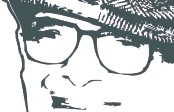
\includegraphics[scale=1.2]{chico.jpg}
	\end{center}
	\fi
\end{song}


\begin{song}{Súplica à Jesus}{C}
  {Desconhecido}
  {Adriano Gomes}
  {}
  {\NotCCLIed}
  
	\renewcommand{\RevDate}{11 de maio de 2015}

	\SBIntro[N]{\Ch{C}{} \Ch{G/B}{} \Ch{Am}{} \Ch{Em}{} \Ch{F}{} \Ch{Fm}{} \Ch{C}{} \Ch{G7}{}}
  
	\ifChordBk
	  {\vspace{-2em}\flushright{\Gchord \quad \GBchord \quad \Amchord \quad \Emchord \quad \Fchord \quad \Fmchord
	  
	  ~ \\
	  
	  \Cchord \quad \Gschord}\\}
	  \vspace{-4ex}
	\fi
  
	\begin{SBVerse*}
		Je\Ch{C}{sus}, no silêncio da \Ch{G/B}{}prece
		
		Teus \Chr{Am}{ir}mãos a Ti pedem \Ch{Em}{paz}
		
		P'ra \Ch{F}{a}liviar um \Ch{Fm}{} pouco as afli\Ch{C}{ções} \Ch{G7}{}
		
		Se\Ch{C}{nhor}, enxugai nosso \Ch{G/B}{pra}nto
		
		Pre\Chr{Am}{ci}samos do Teu a\Ch{Em}{mor}
		
		E \Ch{F}{sen}tir Tua pre\Ch{Fm}{sen}ça
		
		Envol\Ch{C}{ver} \Ch{G/B}{nos}sos cora\Ch{Am}{ções}
		
		\Ch{F}{} Por isso vem,\Ch{G}{} Jesus \Ch{C}{} \Ch{C7}{}
	\end{SBVerse*}
	
	\begin{SBVerse*}
	\begin{SBBracket}{bis}
		E \Ch{F}{ir} ao Teu en\Ch{Em}{con}tro
		
		Que\Ch{F}{re}mos Te segu\Ch{C}{ir} \Ch{G/B}
		
		E afas\Ch{Am}{tar} o mal da \Ch{Em}{Ter}ra
		
		E \Ch{Am}{aca}bar de vez a \Ch{Em}{guer}ra
		
		E ca\Ch{F}{mi}nharmos \Ch{G}{jun}tos rumo \Ch{C}{} à luz \Ch{C7}{}
	\end{SBBracket}
	\end{SBVerse*}

	\begin{SBVerse*}
%		\begin{SBBracket}{2x}
			E ca\Ch{F}{mi}nharmos \Ch{G}{jun}tos rumo \Ch{Fm}{} à luz \Ch{C}{}
%		\end{SBBracket}
	\end{SBVerse*}
\end{song}


\begin{song}{Te Ofereço Paz}{C}
  {Grupo Sal da Terra}
  {Grupo Sal da Terra}
  {}
  {\NotCCLIed}
  
	\renewcommand{\RevDate}{28 de abril de 2015}
 
	\SBIntro[N]{\Ch{C}{} \Ch{F}{} \Ch{Em}{} \Ch{Dm}{} \Ch{G7}{} \Ch{C}{}}
	
	% As cifras alinhadas à direita
	\ifChordBk	
		\vspace{-2em}\flushright{\Cchord \quad \Cschord \quad \Fchord \quad \Emchord 
				\quad \Dmchord \quad \Gschord}
		\vspace{-1ex}
	\fi
	
	\begin{SBVerse*}
	
	\Ch{C}{}Te ofereço \Ch{F}{paz}

	\Ch{Em}{}Te ofereço \Ch{~~Dm}{Amor}

	\Ch{G7}{}Te ofereço ami\Ch{C}{zade}

	\Ch{C7}{}Ouço tuas necessi\Ch{F}{dades}

	\Ch{Em}{}Vejo tua be\Ch{Dm}{leza}

	\Ch{G7}{}Sinto os teus senti\Ch{C}{mentos}\Ch{C7}{}

	\Ch{F}{Minha} sabedo\Ch{Em}{ria} flui \Ch{Am}{}

	\Ch{Dm}{De} uma \Ch{G7}{fonte} su\Ch{C}{perior}

	\Ch{F}{E} reconheço essa \Ch{Em}{fonte} em \Ch{Am}{Ti}

	\Ch{Dm}{Tra}ba\Ch{G7}{lhe}mos jun\Ch{C}{tos} 

	\Ch{Dm}{Tra}ba\Ch{G7}{lhe}mos jun\Ch{C}{tos} 
	\end{SBVerse*}
\end{song}



\begin{song}{Vem Com a Gente}{D}
  {Violão Amigo}
  {Anderson Mattos e Elias}
  {}
  {\NotCCLIed}
  
	\renewcommand{\RevDate}{12 de junho de 2015}
 
	\SBIntro[N]{\Ch{D}{} \Ch{G}{} \Ch{D}{} \Ch{G}{} \Ch{D}{} \Ch{G}{} \Ch{A}{}}
	
	% As cifras alinhadas à direita
	\ifChordBk	
		\vspace{-2em}\flushright{\Dchord \quad \Achord \quad \Gchord \quad \Emchord \quad \Bmchord \quad \Dschord \quad \Gbmchord}
		\vspace{-1ex}
	\fi
	
	\begin{SBVerse}
		\Ch{D}{Vem}, vem com \Ch{G}{a} gente vem \Ch{D}{amigo}
		
		Traga \Ch{G}{logo} o seu \Ch{D}{} sorriso
		
		Vem sen\Ch{G}{tir} esta \Ch{A}{emoção} \Ch{G}{} ~ \Ch{A}{}
		
	\end{SBVerse}
	
	\begin{minipage}{0.6\columnwidth}
	\flushright
	\begin{SBVerse}
		\Ch{D}{Vem}, vem com \Ch{G}{a} gente vem \Ch{D}{cantar}
		
		Semear\Ch{G}{} flores de \Ch{D}{alegria}
		
		Vem com a \Ch{G}{gente} e\Ch{A}{vangeli}\Ch{G}{zar} \Ch{A}{}
	\end{SBVerse}
	\end{minipage}
	
	\begin{SBVerse}
		\Ch{G}{Juntos} no com\Ch{A}{passo} desse \Ch{Gbm}{} violão
		
		Vamos \Ch{Bm}{espalhar} nossa \Ch{Em}{} canção
		
		\Ch{A}{Ver} o amor desabro\Ch{D}{char}
		
		Em cada \Ch{D7}{}coração
	\end{SBVerse}
	
	\begin{minipage}{0.6\columnwidth}
	\vspace{-2ex}
	\flushright
	\begin{SBVerse}
		\Ch{G}{Vem}, \Ch{A}{com} o Violão Amigo \Ch{G}{} vem
		
		\Ch{A}{Vem} com a gente, amigo, \Ch{G}{} vem
		
		Vem \Ch{A}{e} traga essa \Ch{B}{} luz que existe em \Ch{G}{você}
		
		que existe em \Ch{A}{você}

		{\normalsize\texttt{\textbf{(Repete tudo 1x)}}}
	\end{SBVerse}
	\end{minipage}
		
	\begin{SBVerse*}
		(1ª) \Ch{G}{Vem,} vamos \Ch{A}{lá} fazer bri\Ch{G}{lhar}
		
		(2ª) Vamos \Ch{A}{lá} fazer bri\Ch{G}{lhar}
		
		(3ª) Vamos \Ch{A}{lá} fazer bri\Ch{B}{lhar}... \Ch{G}{Fazer} brilhar... \Ch{A}{brilhar...} \Ch{D}{brilhar}

		\flushright\begin{SBBracket}{Final}
			\hspace*{-3cm} Vem com a gente, vem! (falado)
		\end{SBBracket}
	\end{SBVerse*}
\end{song}


\begin{song}{Vogais}{G}
  {Concafras}
  {Desconhecido}
  {}
  {\NotCCLIed}
  
	\renewcommand{\RevDate}{17 de setembro de 2015}
 
	\SBIntro[N]{\Ch{G}{} \Ch{Em}{} \Ch{C}{} \Ch{D}{}}
	
	% As cifras alinhadas à direita
	\ifChordBk	
		\vspace{-2em}\flushright{\Gchord \quad \Emchord \quad \Cchord \quad \Dchord}
		\vspace{-1ex}
	\fi
	
	\begin{SBVerse*}
	
		\ifChordBk
			\texttt{{\small (G Em C D)}}
		\fi
	
		Com A eu tenho alegria de montão
		
		Com E eu sinto em mim uma energização
		
		O I me mostra a importância de doar
		
		Sinto orgulho de ser útil e me dedicar
		
		Ah! como é bom trabalhar (2x)

		Ah! como é bom trabalhar
	
		\ifChordBk
			\texttt{{\small (C D G Em)}}
		\fi
		
%		\ifChordBk
%			\texttt{{\small (G Em C D)}}
%		\fi
	
		A, E, I, O, U... eu trabalho pra chuchu
		
		U, O, I, E, A... trabalhando com o coração, aprendo a amar
		
		A, E, I, O, U... eu trabalho pra chuchu
		
		U, O, I, E, A... trabalhando com o coração, aprendo a amar (2x)
	\end{SBVerse*}
\end{song}



\begin{song}{Voz do Coração}{D}
  {A pesquisar}
  {A pesquisar}
  {}
  {\NotCCLIed}
  
	\renewcommand{\RevDate}{20 de agosto de 2015}
 
	\SBIntro[N]{\Ch{C7+}{} \Ch{Fm7+}{} \Ch{C7+}{} \Ch{Fm7+}{} }
	
	% As cifras alinhadas à direita
	\ifChordBk	
		\vspace{-2em}\flushright{\Csaumchord \quad \Fmsaumchord \quad \Fchord \quad \Gschord}
		\vspace{-1ex}
	\fi
	
%	\begin{SBVerse*}
		\begin{SBBracket}{2x}
			\ifChordBk	
			{\normalsize \texttt{\textbf{(C7+ Fm7+ C7+ Fm7+)}}}
			\fi
			
%			\Ch{C7+}{}Quando a gente quer \Ch{Fm7+}{}ouvir um \Ch{C7+}{}coração \Ch{Fm7+}{}

			Quando a gente quer ouvir um coração

			Para descobrir a fonte do amor
			
			\Ch{F}{}Que vai nos \Ch{G7}{fazer} mais leves
			
			\ifChordBk	
			{\normalsize \texttt{\textbf{(C7+ Fm7+ C7+ Fm7+)}}}
			\fi
			
			Mais fortes pra crescer
			
			Quando a gente quer as vezes dói
			
			É olhar pra dentro bem nos olhos
			
			Desvendar mistérios desatar mil nós
			
			\Ch{F}{}Pra sair num \Ch{G7}{voo} lindo
			
			\ifChordBk	
			{\normalsize \texttt{\textbf{(C7+ Fm7+ C7+ Fm7+)}}}
			\fi

			E encontrar um outro irmão
			
			E dizer bem vindo no meu coração
		\end{SBBracket}

		\begin{SBVerse*}
			\ifChordBk	
			{\normalsize \texttt{\textbf{(C7+ Fm7+ C7+ Fm7+)}}}
			\fi
			\quad no meu coração ~ \texttt{(3x)}
		\end{SBVerse*}	
%	\end{SBVerse*}
	
\end{song}


%%Uma nova música - copie, cole, descomente e edite
%\begin{song}{Nome da música}{Tom}
%  {Copyright}
%  {Autoria e Música}
%  {}
%  {\NotCCLIed}
%  
%	\renewcommand{\RevDate}{12 de maio de 2014}
% 
%	\SBIntro[N]{\Ch{D}{} \Ch{G}{} \Ch{A7}{} \Ch{D}{}}
%	
%	% As cifras alinhadas à direita
%	\ifChordBk	
%		\vspace{-2em}\flushright{\Gchord \quad \Cchord}
%		\vspace{-1ex}
%	\fi
%	
%	%Uma estrofe sem numeracao
%	\begin{SBVerse*}
%		Uma estrofe
%		
%		sem numeração
%	\end{SBVerse*}
%  
%	%Uma estrofe numerada
%	\begin{SBVerse}
%		Uma estrofe
%		
%		numerada
%	\end{SBVerse}
%
%	%Um grupo aberto
%	\begin{SBOpGroup}
%		Um grupo
%		
%		aberto
%	\end{SBOpGroup}
%	
%	%Uma parte com destaque
%	\begin{SBBracket}{bis}
%		Uma parte com destaque
%		
%		bla bla bla
%	\end{SBBracket}
%	
%	%Refrão
%	\begin{SBChorus}
%		Use \verb+\Ch{D}{+\Ch{D}{pa}\}ra colocar acordes normais
%		
%		Use \verb+\Chr{D/F#}{+\Chr{D/F#}{pa\}}ra colocar uma ligadura
%	\end{SBChorus}
%	
%	\newpage
%	
%	%Refrão sem a tag
%	\begin{SBChorus*}
%		bla bla bla
%		
%		bla bla bla
%	\end{SBChorus*}
%	
%	%Usar multicolum para duas colunas alinhas
%	\begin{multicols}{2}
%		Este texto estará espalhado em duas colunas 
%		uniformemente distribuídas. Para forçar 
%		uma quebra de coluna use \verb+\columnbreak+
%	\end{multicols}
%	
%	
%	%Usar minipage para duas colunas alinhas independentemente
%	\flushleft{}
%	
%	\begin{minipage}{0.5\textwidth}
%		versos alinhados à esquerda
%		
%		na primeira coluna
%		
%		alinhada no topo
%	\end{minipage}
%	
%	\vspace{-3em}
%	
%	\flushright{}
%	
%	\begin{minipage}{0.5\textwidth}
%		\vfill
%		
%		versos alinhados à esquerda
%		
%		na segunda coluna
%		
%		alinhada na base
%	\end{minipage}
%\end{song}



% Indice das musicas
\cleardoublepage
\thispagestyle{empty}
{\Large \textbf{Índice das Músicas}}
\begin{description}
\item\ 1. A can\IeC {\c c}\IeC {\~a}o que a gente fez\hbox {, 1}
\item\ 2. Al\IeC {\c c}ar voo\hbox {, 2}
\item\ 3. Amanhecer\hbox {, 3}
\item\ 4. A Paz\hbox {, 4}
\item\ 5. Bem Aqui Onde Estou\hbox {, 5}
\item\ 6. Boa Nova\hbox {, 6}
\item\ 7. Boa Nova\hbox {, 7}
\item\ 8. Brilhem Mais\hbox {, 8}
\item\ 9. Can\IeC {\c c}\IeC {\~a}o da Alegria Crist\IeC {\~a}\hbox {, 9}
\item\ 10. Casa Torta\hbox {, 10}
\item\ 11. Cativar\hbox {, 11}
\item\ 12. Coisas Pequeninas\hbox {, 12}
\item\ 13. Como \IeC {\'e} Grande o Meu Amor por Voc\IeC {\^e}\hbox {, 13}
\item\ 14. D\IeC {\^e} um sorriso (sequ\IeC {\^e}ncia)\hbox {, 14}
\item\ 15. Dia das M\IeC {\~a}es\hbox {, 16}
\item\ 16. Encontro Marcado\hbox {, 17}
\item\ 17. Esp\IeC {\'\i }rito Imortal\hbox {, 18}
\item\ 18. Jesus\hbox {, 19}
\item\ 19. Lembre-se\hbox {, 20}
\item\ 20. Liberdade\hbox {, 21}
\item\ 21. Luz da Vida\hbox {, 22}
\item\ 22. Luzes\hbox {, 23}
\item\ 23. N\IeC {\~a}o \IeC {\'e} Mole N\IeC {\~a}o\hbox {, 24}
\item\ 24. O Belo\hbox {, 25}
\item\ 25. O Essencial\hbox {, 26}
\item\ 26. O Natal Existe\hbox {, 27}
\item\ 27. Obrigado Criador\hbox {, 28}
\item\ 28. Pai Nosso\hbox {, 29}
\item\ 29. Para Sempre Em Meu Cora\IeC {\c c}\IeC {\~a}o\hbox {, 30}
\item\ 30. Pedacinho de Luar\hbox {, 32}
\item\ 31. Prece\hbox {, 33}
\item\ 32. Poeta Jesus\hbox {, 34}
\item\ 33. Quando Te Vi\hbox {, 35}
\item\ 34. Quem \IeC {\'e} feliz\hbox {, 36}
\item\ 35. Reencarna\IeC {\c c}\IeC {\~a}o\hbox {, 37}
\item\ 36. Sentir Deus\hbox {, 38}
\item\ 37. Sentir Jesus\hbox {, 39}
\item\ 38. Ser Feliz e Amar\hbox {, 40}
\item\ 39. S\IeC {\'u}plica \IeC {\`a} Jesus\hbox {, 42}
\item\ 40. Te Ofere\IeC {\c c}o Paz\hbox {, 43}
\item\ 41. Vem Com a Gente\hbox {, 44}
\item\ 42. Vogais\hbox {, 45}
\item\ 43. Voz do Cora\IeC {\c c}\IeC {\~a}o\hbox {, 46}

\end{description}

\newpage
\thispagestyle{empty}
\mbox{}

\end{document}
\bye
%
%%%
% Document ends.
%%%
